\section*{Глава 2. Проектирование веб-приложения}
\addcontentsline{toc}{section}{Глава 2. Проектирование веб-приложения}
\stepcounter{section}

\subsection{Анализ целевой аудитории}

Разрабатываемое веб-приложение предназначено для автоматизации процессов
документооборота и управления мероприятиями в культурно-досуговых
учреждениях. Основными пользователями системы являются сотрудники
учреждения, участвующие в организации, согласовании и сопровождении
мероприятий.

В системе выделяются следующие основные роли пользователей:

\begin{itemize}
	\item \textbf{Сотрудник} --- базовый пользователь системы, осуществляющий
	      работу с карточками мероприятий, документами и отчетностью.

	\item \textbf{Руководитель СП} --- пользователь, ответственный за создание
	      мероприятий, назначение ответственных сотрудников и контроль
	      выполнения задач. Руководитель структурного подразделения.

	\item \textbf{Художественный руководитель} --- пользователь, выполняющий
	      согласование или отклонение мероприятий, а также формирование
	      статистики и отчетности.

	\item \textbf{ИТ-администратор} --- пользователь, осуществляющий управление
	      учетными записями, ролями и правами доступа.
\end{itemize}

При проектировании интерфейса учитывались особенности работы сотрудников
культурно-досуговых учреждений: необходимость быстрого доступа к
документам, минимизация количества действий при работе с мероприятиями,
а также простота освоения системы без длительного обучения.

\newpage
\subsection{Описание функциональности приложения}

Функциональность системы определяется процессами создания, согласования
и сопровождения мероприятий, а также хранением связанной документации.

2 Основных сценария использования системы могут быть представлены в виде
следующих User Story:

\textit{«Я, как руководитель структурного подразделения, хочу создавать
карточки мероприятий, указывать их категорию, дату проведения,
ответственного сотрудника и плановые показатели, чтобы информация
о мероприятиях хранилась централизованно и могла использоваться
для последующего формирования отчётности».}

\textit{«Я, как художественный руководитель, хочу просматривать сведения
о проведённых мероприятиях, количестве посетителей и полученных
внебюджетных средствах за выбранный период, чтобы оперативно
формировать ежемесячные отчёты и контролировать результаты работы
учреждения».}

Система предоставляет следующие функциональные возможности:

\begin{itemize}
	\item авторизация пользователей;
	\item создание и редактирование карточек мероприятий;
	\item назначение ответственных сотрудников;
	\item согласование и отклонение мероприятий;
	\item загрузка и хранение документов;
	\item формирование статистики и отчетности;
	\item выгрузка документов и отчетов;
	\item управление учетными записями и ролями пользователей.
\end{itemize}

На рисунке~\ref{fig:use_case} представлена диаграмма вариантов
использования системы.

\begin{figure}[ht!]
	\centering
	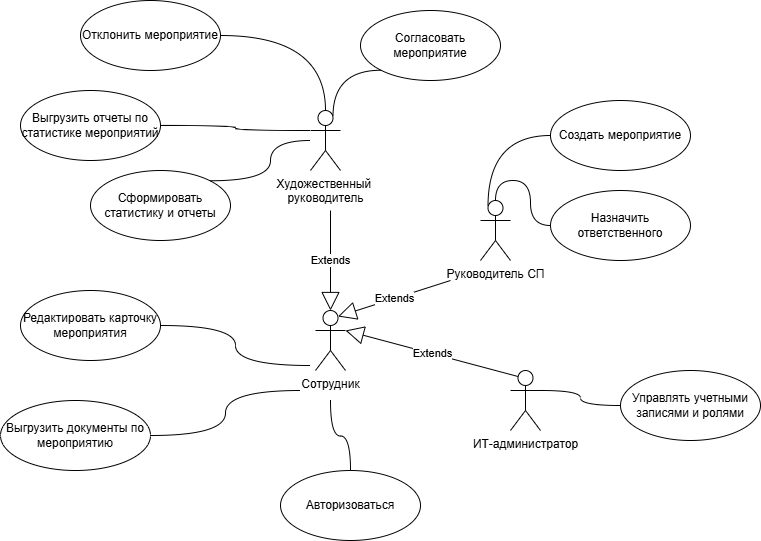
\includegraphics[width=0.95\textwidth]{images/usecase_diagram.png}
	\caption{Диаграмма вариантов использования системы}
	\label{fig:use_case}
\end{figure}

\clearpage
\subsection{Проектирование модели данных}
Для хранения данных приложения выбрана реляционная модель данных на
основе СУБД PostgreSQL. Использование реляционной базы данных позволяет
обеспечить целостность данных, поддержку связей между сущностями и
разграничение прав доступа пользователей.

Основными сущностями системы являются:
\begin{itemize}
	\item пользователи;
	\item роли;
	\item мероприятия;
	\item категории мероприятий;
	\item статусы мероприятий;
	\item файлы.
\end{itemize}
Центральной сущностью системы является мероприятие, содержащее
основную информацию о событии, статусе согласования, категории,
ответственном пользователе и связанных документах.

На рисунке~\ref{fig:er_diagram} представлена ER-диаграмма базы данных.

\begin{figure}[H]
	\centering
	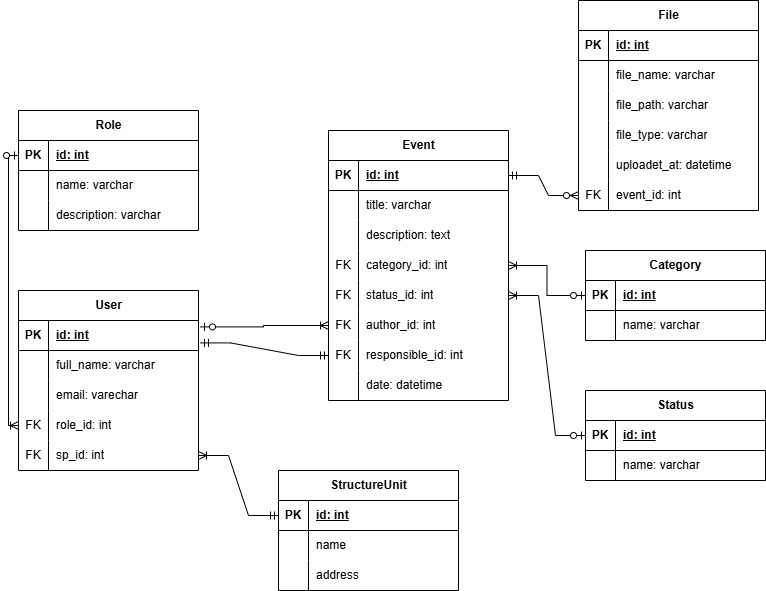
\includegraphics[width=\textwidth]{images/er_diagram.png}
	\caption{ER-диаграмма базы данных}
	\label{fig:er_diagram}
\end{figure}

Структура основной таблицы мероприятий представлена в
таблице~\ref{tab:event_table}.

\begin{longtable}{|p{3.5cm}|p{3cm}|p{7cm}|}
	\caption{Структура таблицы мероприятий (\texttt{event})}
	\label{tab:event_table} \\

	\hline
	\textbf{Поле} & \textbf{Тип данных} & \textbf{Описание} \\ \hline
	\endfirsthead

	\hline
	\textbf{Поле} & \textbf{Тип данных} & \textbf{Описание} \\ \hline
	\endhead

	id & INT & Уникальный идентификатор мероприятия \\ \hline
	title & VARCHAR & Название мероприятия \\ \hline
	description & TEXT & Описание мероприятия \\ \hline
	category\_id & INT & Ссылка на категорию мероприятия \\ \hline
	status\_id & INT & Ссылка на статус мероприятия \\ \hline
	author\_id & INT & Идентификатор автора мероприятия \\ \hline
    responsible\_id & INT & Идентификатор ответственного сотрудника \\ \hline
	date & DATETIME & Дата проведения мероприятия \\ \hline
\end{longtable}

\subsection{Разработка макетов страниц}

На этапе проектирования интерфейса были разработаны макеты основных
страниц веб-приложения, отражающие ключевые пользовательские сценарии.

Основное внимание при проектировании интерфейса уделялось:

\begin{itemize}
	\item простоте навигации;
	\item минимизации количества действий пользователя;
	\item удобству работы с документами и мероприятиями;
	\item единообразию элементов интерфейса;
	\item адаптации интерфейса под различные роли пользователей.
\end{itemize}

В системе предусмотрены следующие основные страницы:

\begin{itemize}
	\item страница авторизации;
	\item список мероприятий;
    \item форма создания мероприятия;
	\item карточка мероприятия;
	\item страница управления пользователями;
	\item страница отчетности.
\end{itemize}

Макеты страниц разрабатывались с помощью простой верстки HTML+CSS.
\begin{figure}[ht!]
	\centering
	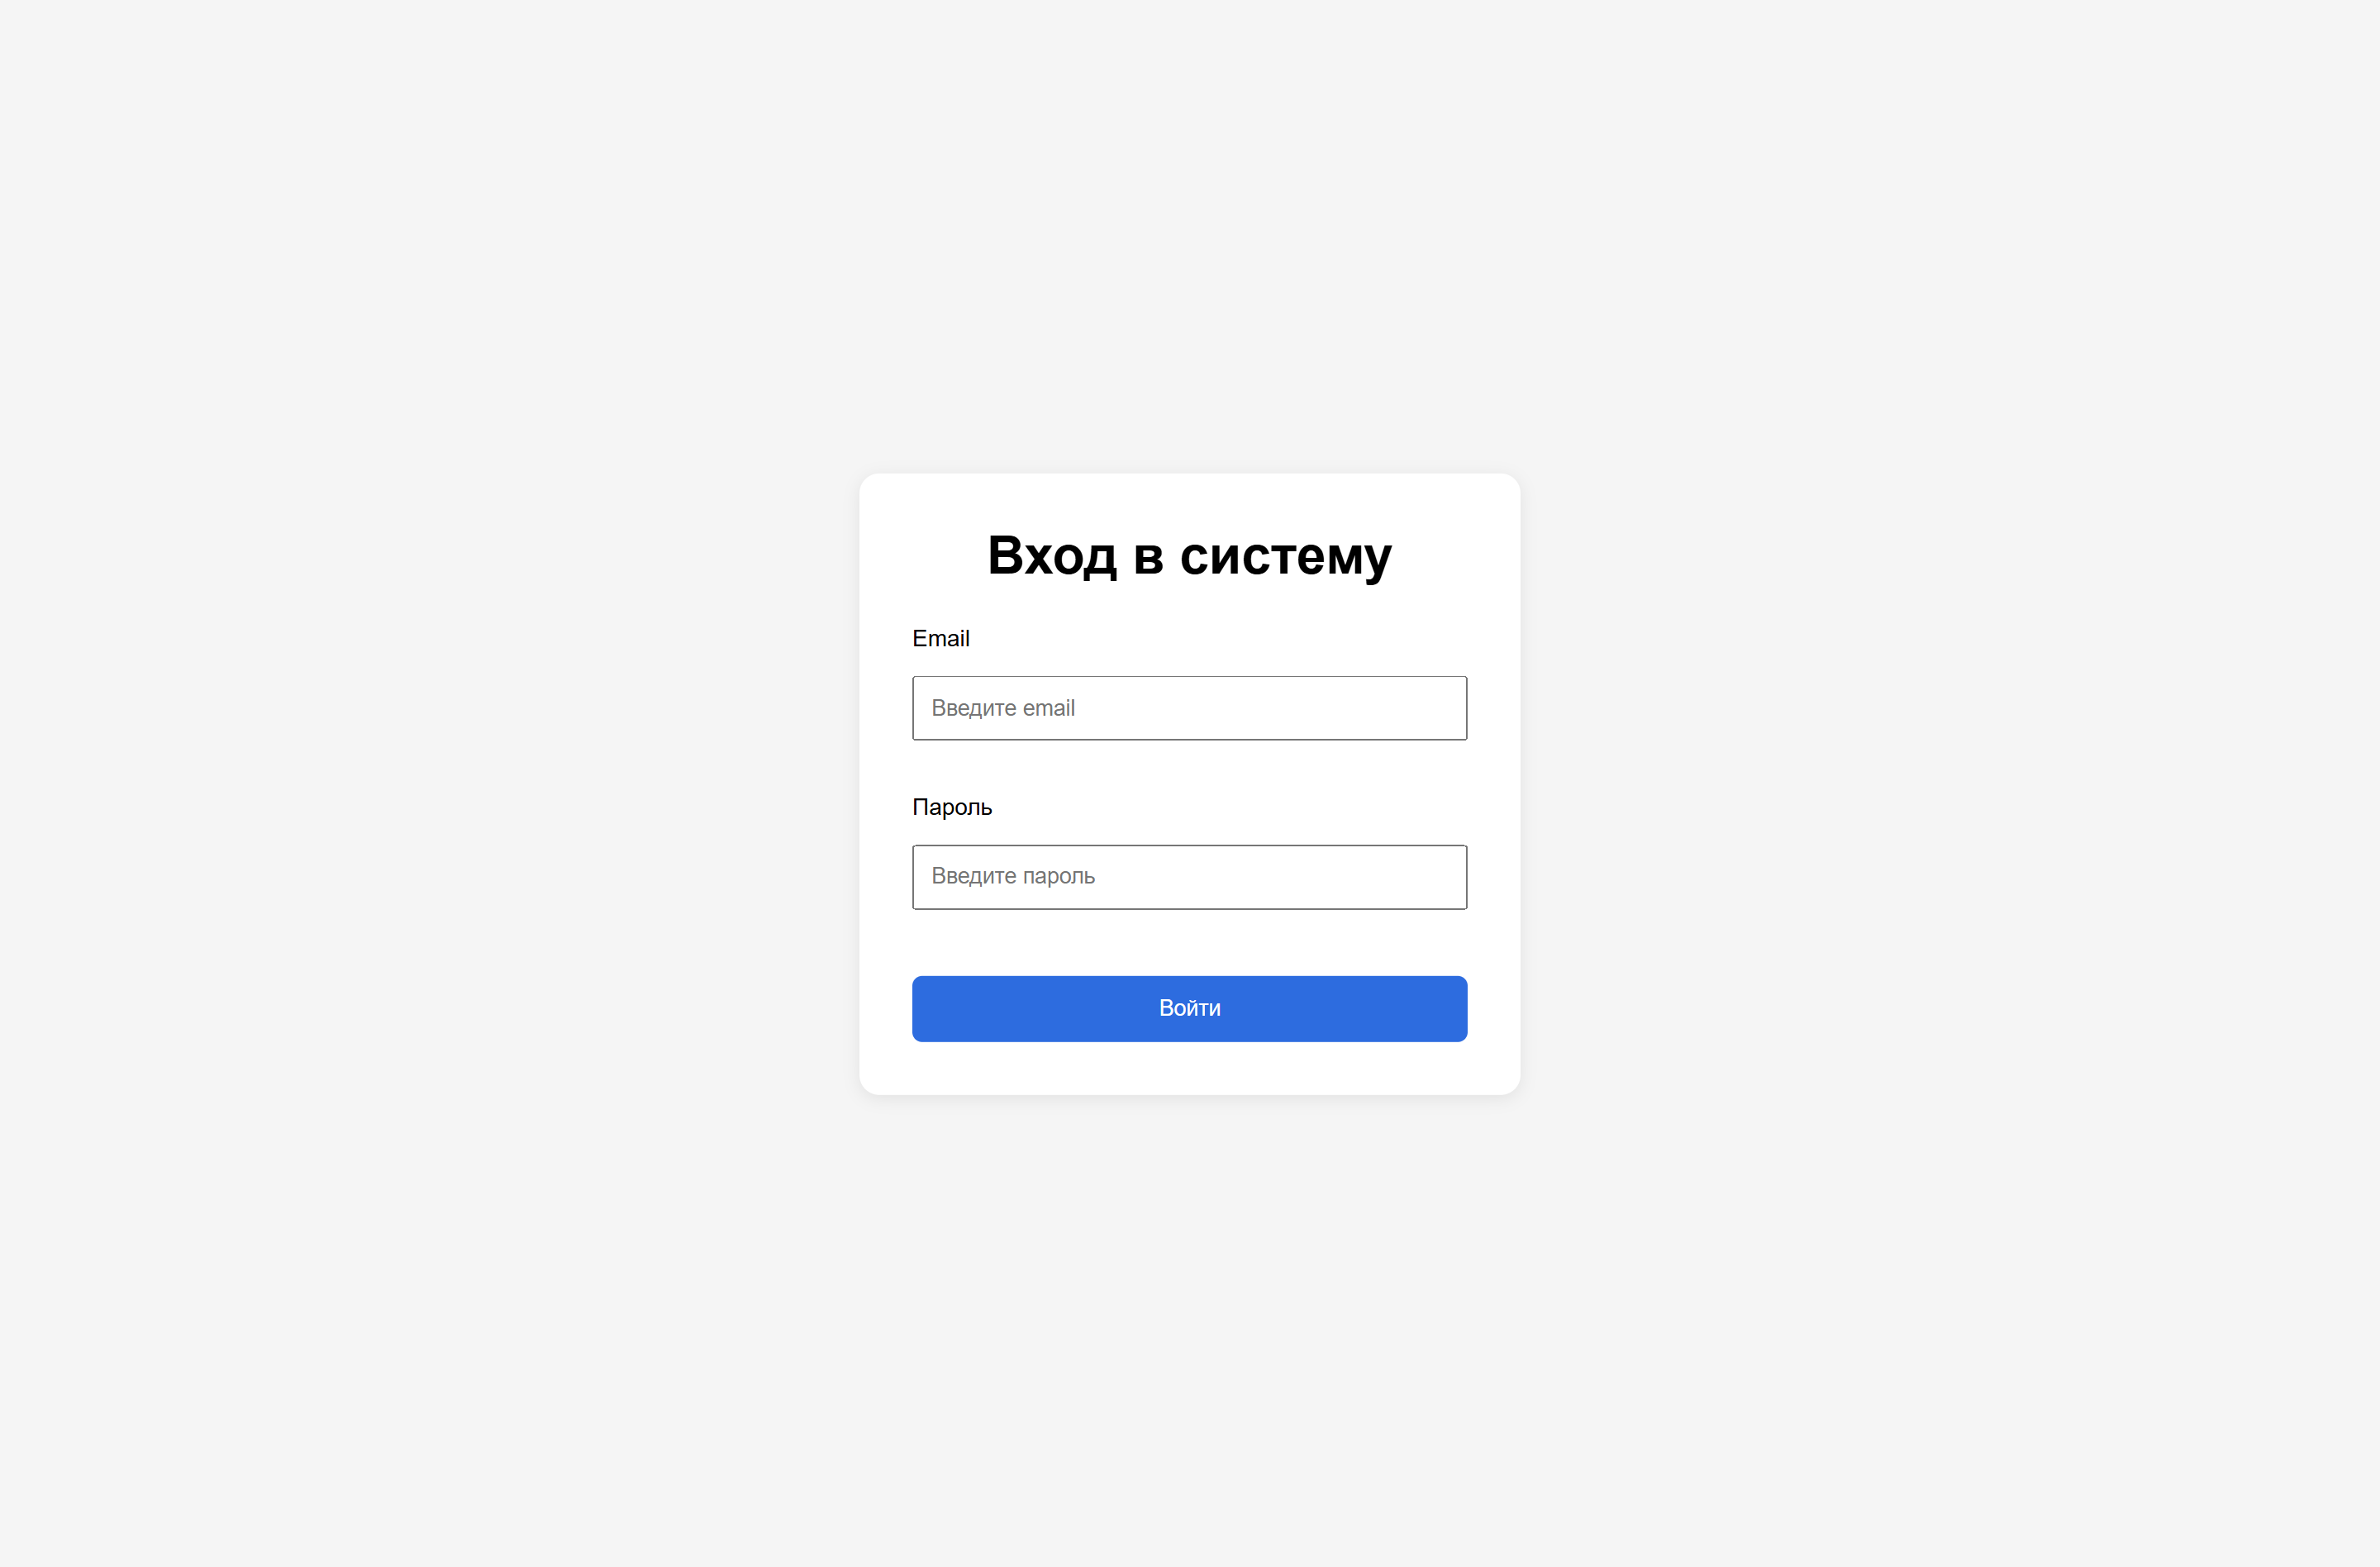
\includegraphics[width=0.95\textwidth]{images/login.png}
	\caption{Страница авторизации}
	\label{fig:use_case}
\end{figure}
\begin{figure}[ht!]
	\centering
	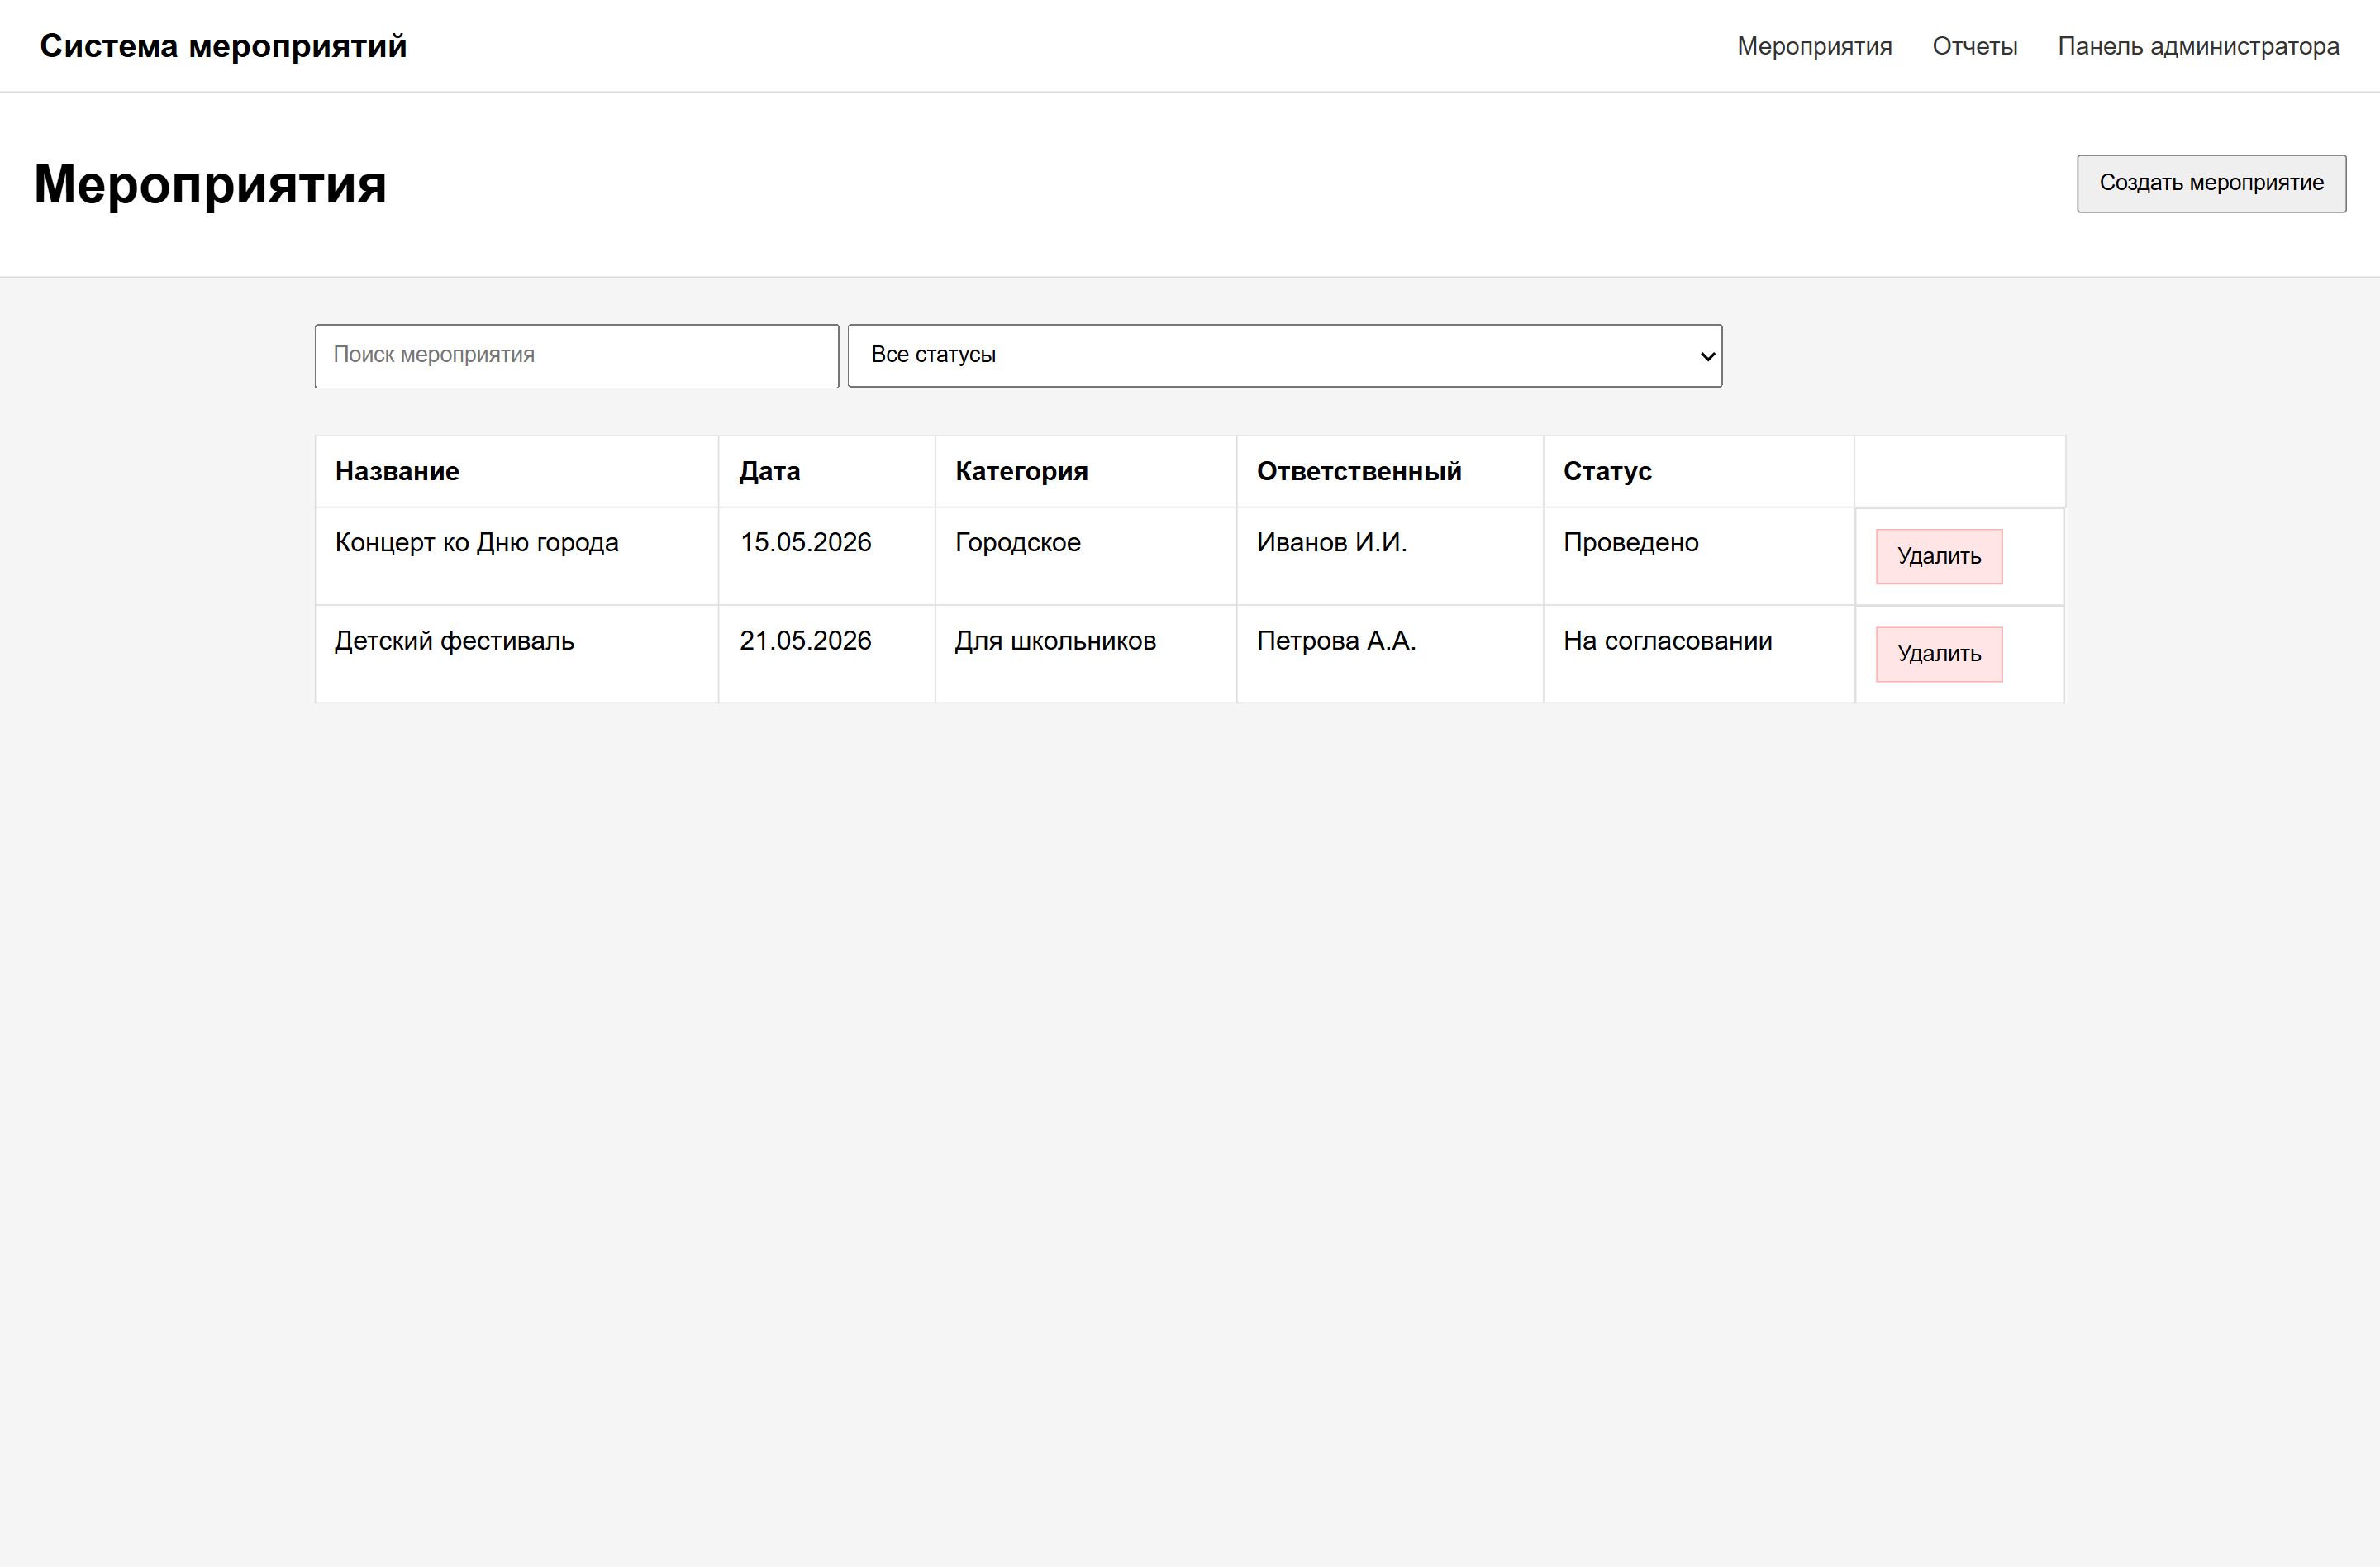
\includegraphics[width=0.95\textwidth]{images/events-list.png}
	\caption{Главная страница со списком мероприятий}
	\label{fig:use_case}
\end{figure}
\begin{figure}[ht!]
	\centering
	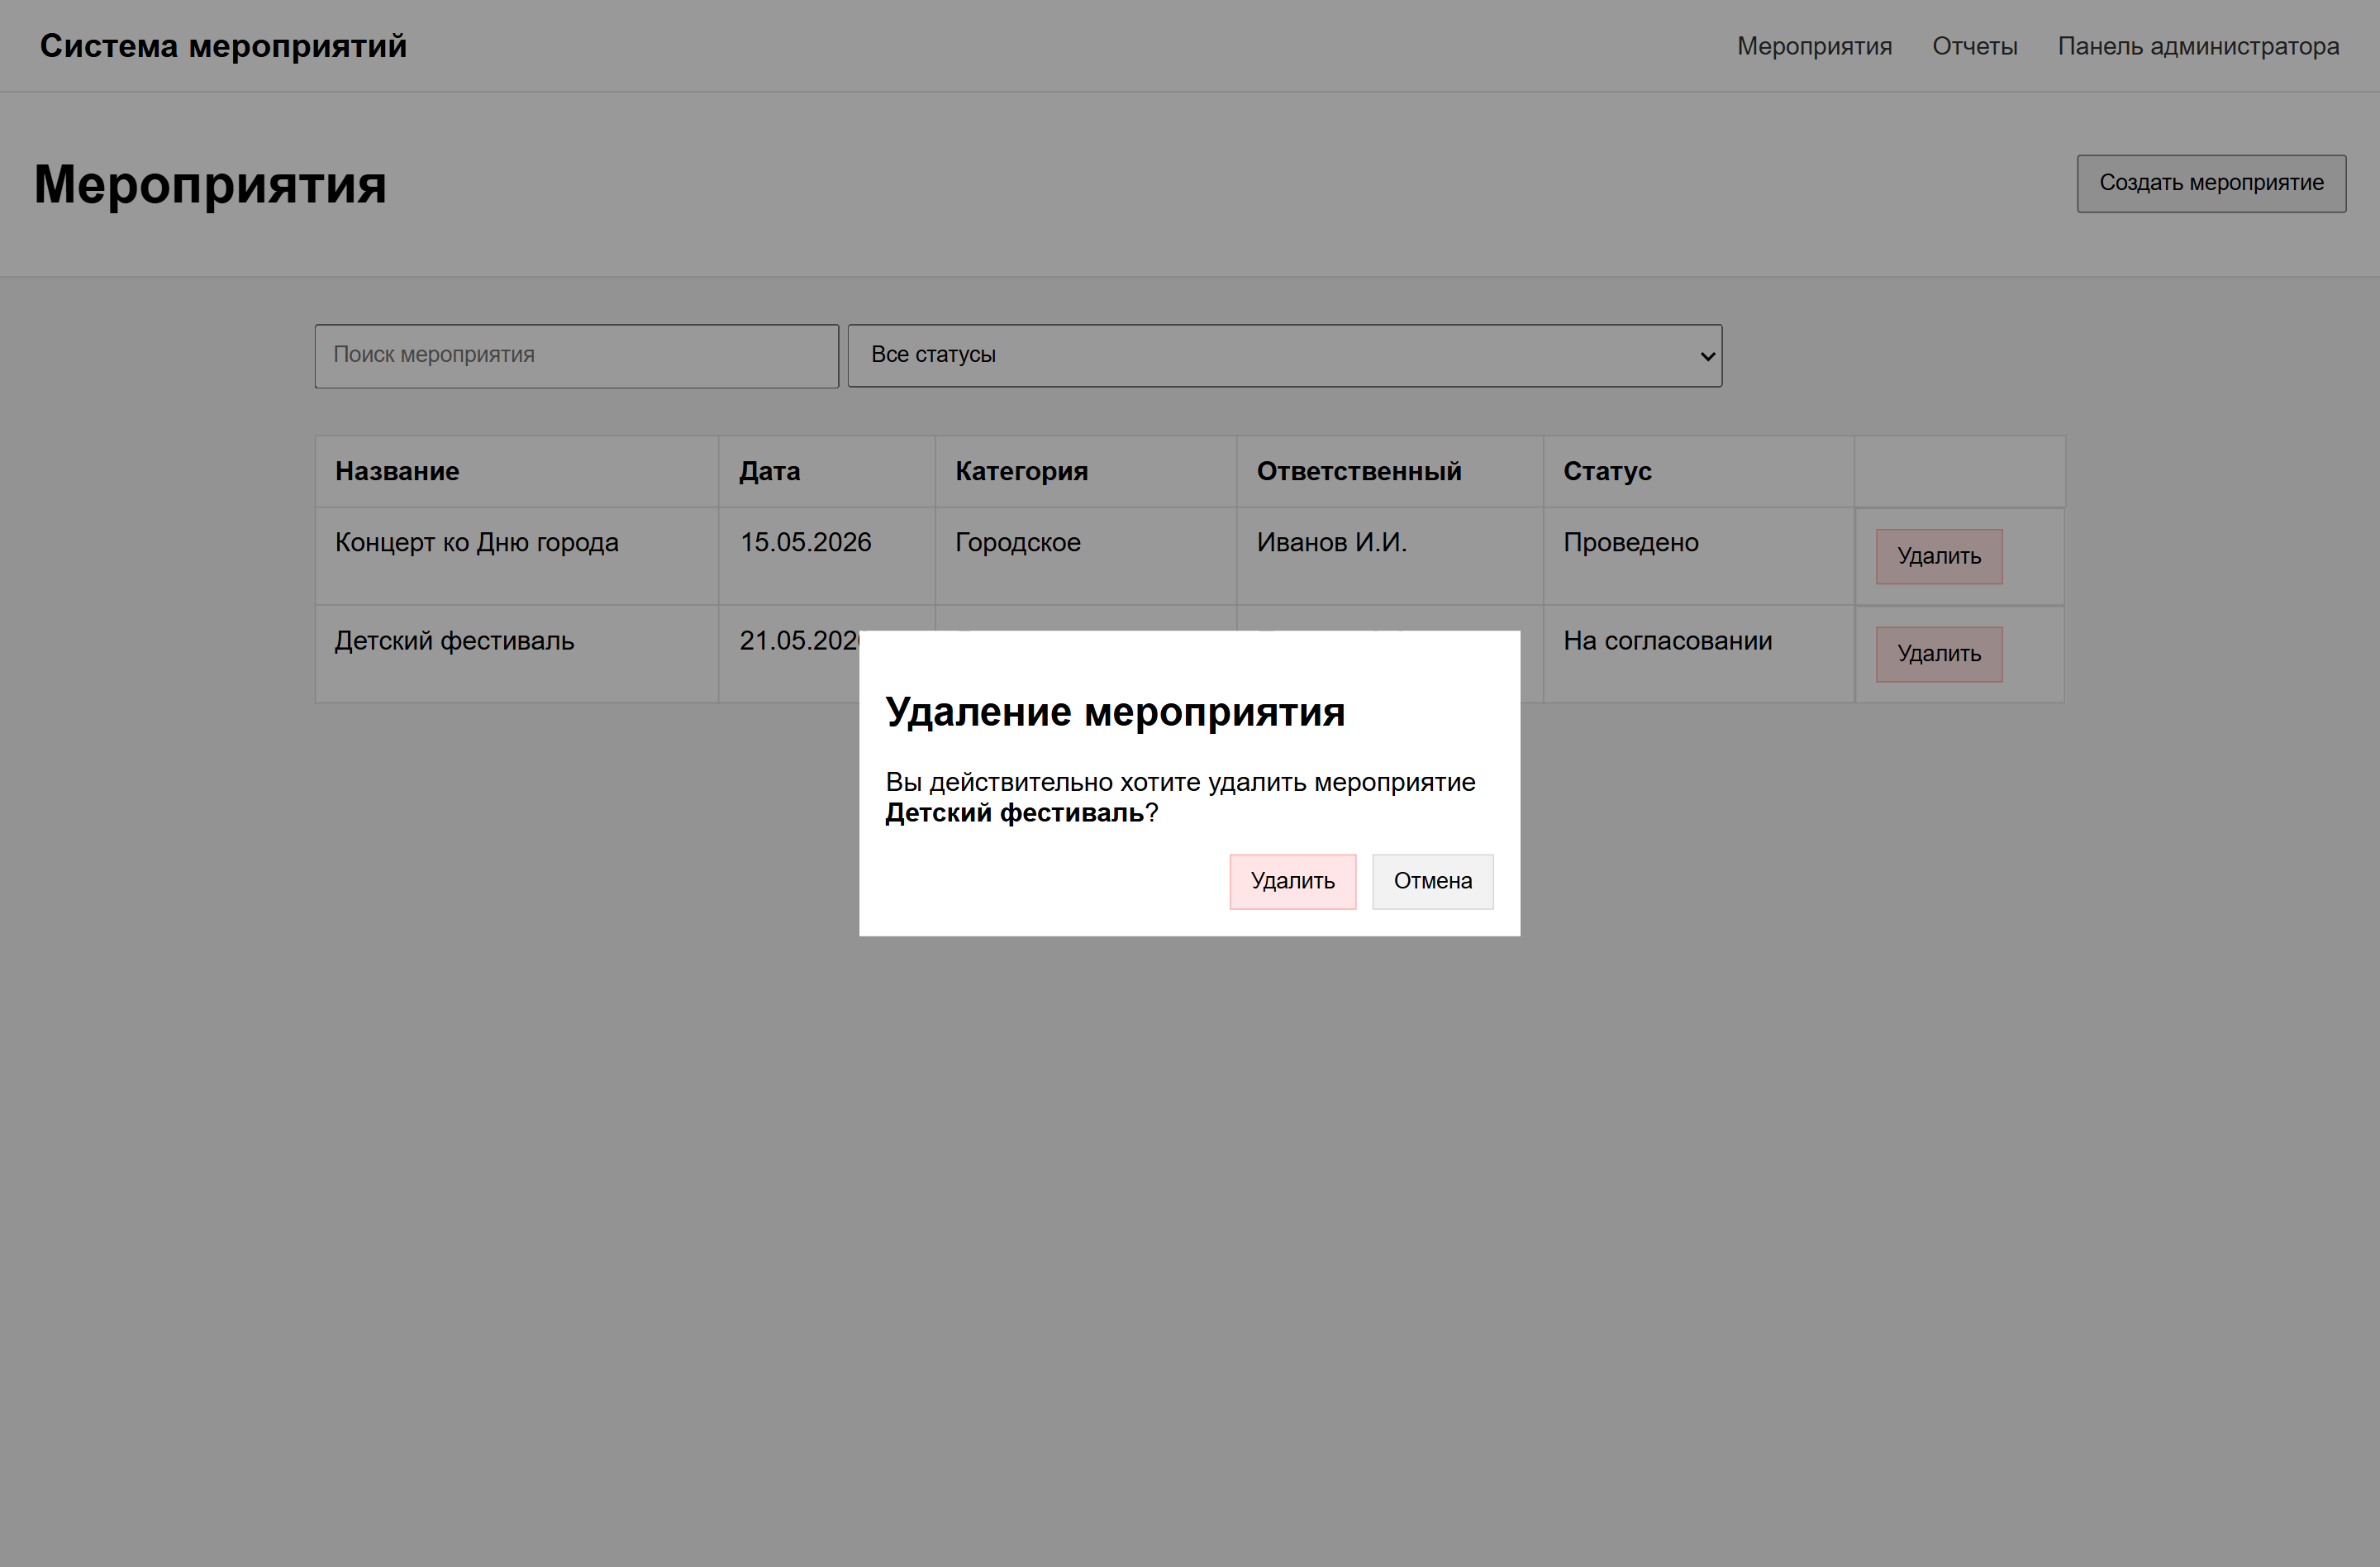
\includegraphics[width=0.95\textwidth]{images/events-list-delete.png}
	\caption{Модальное окно удаления мероприятия}
	\label{fig:use_case}
\end{figure}
\begin{figure}[ht!]
	\centering
	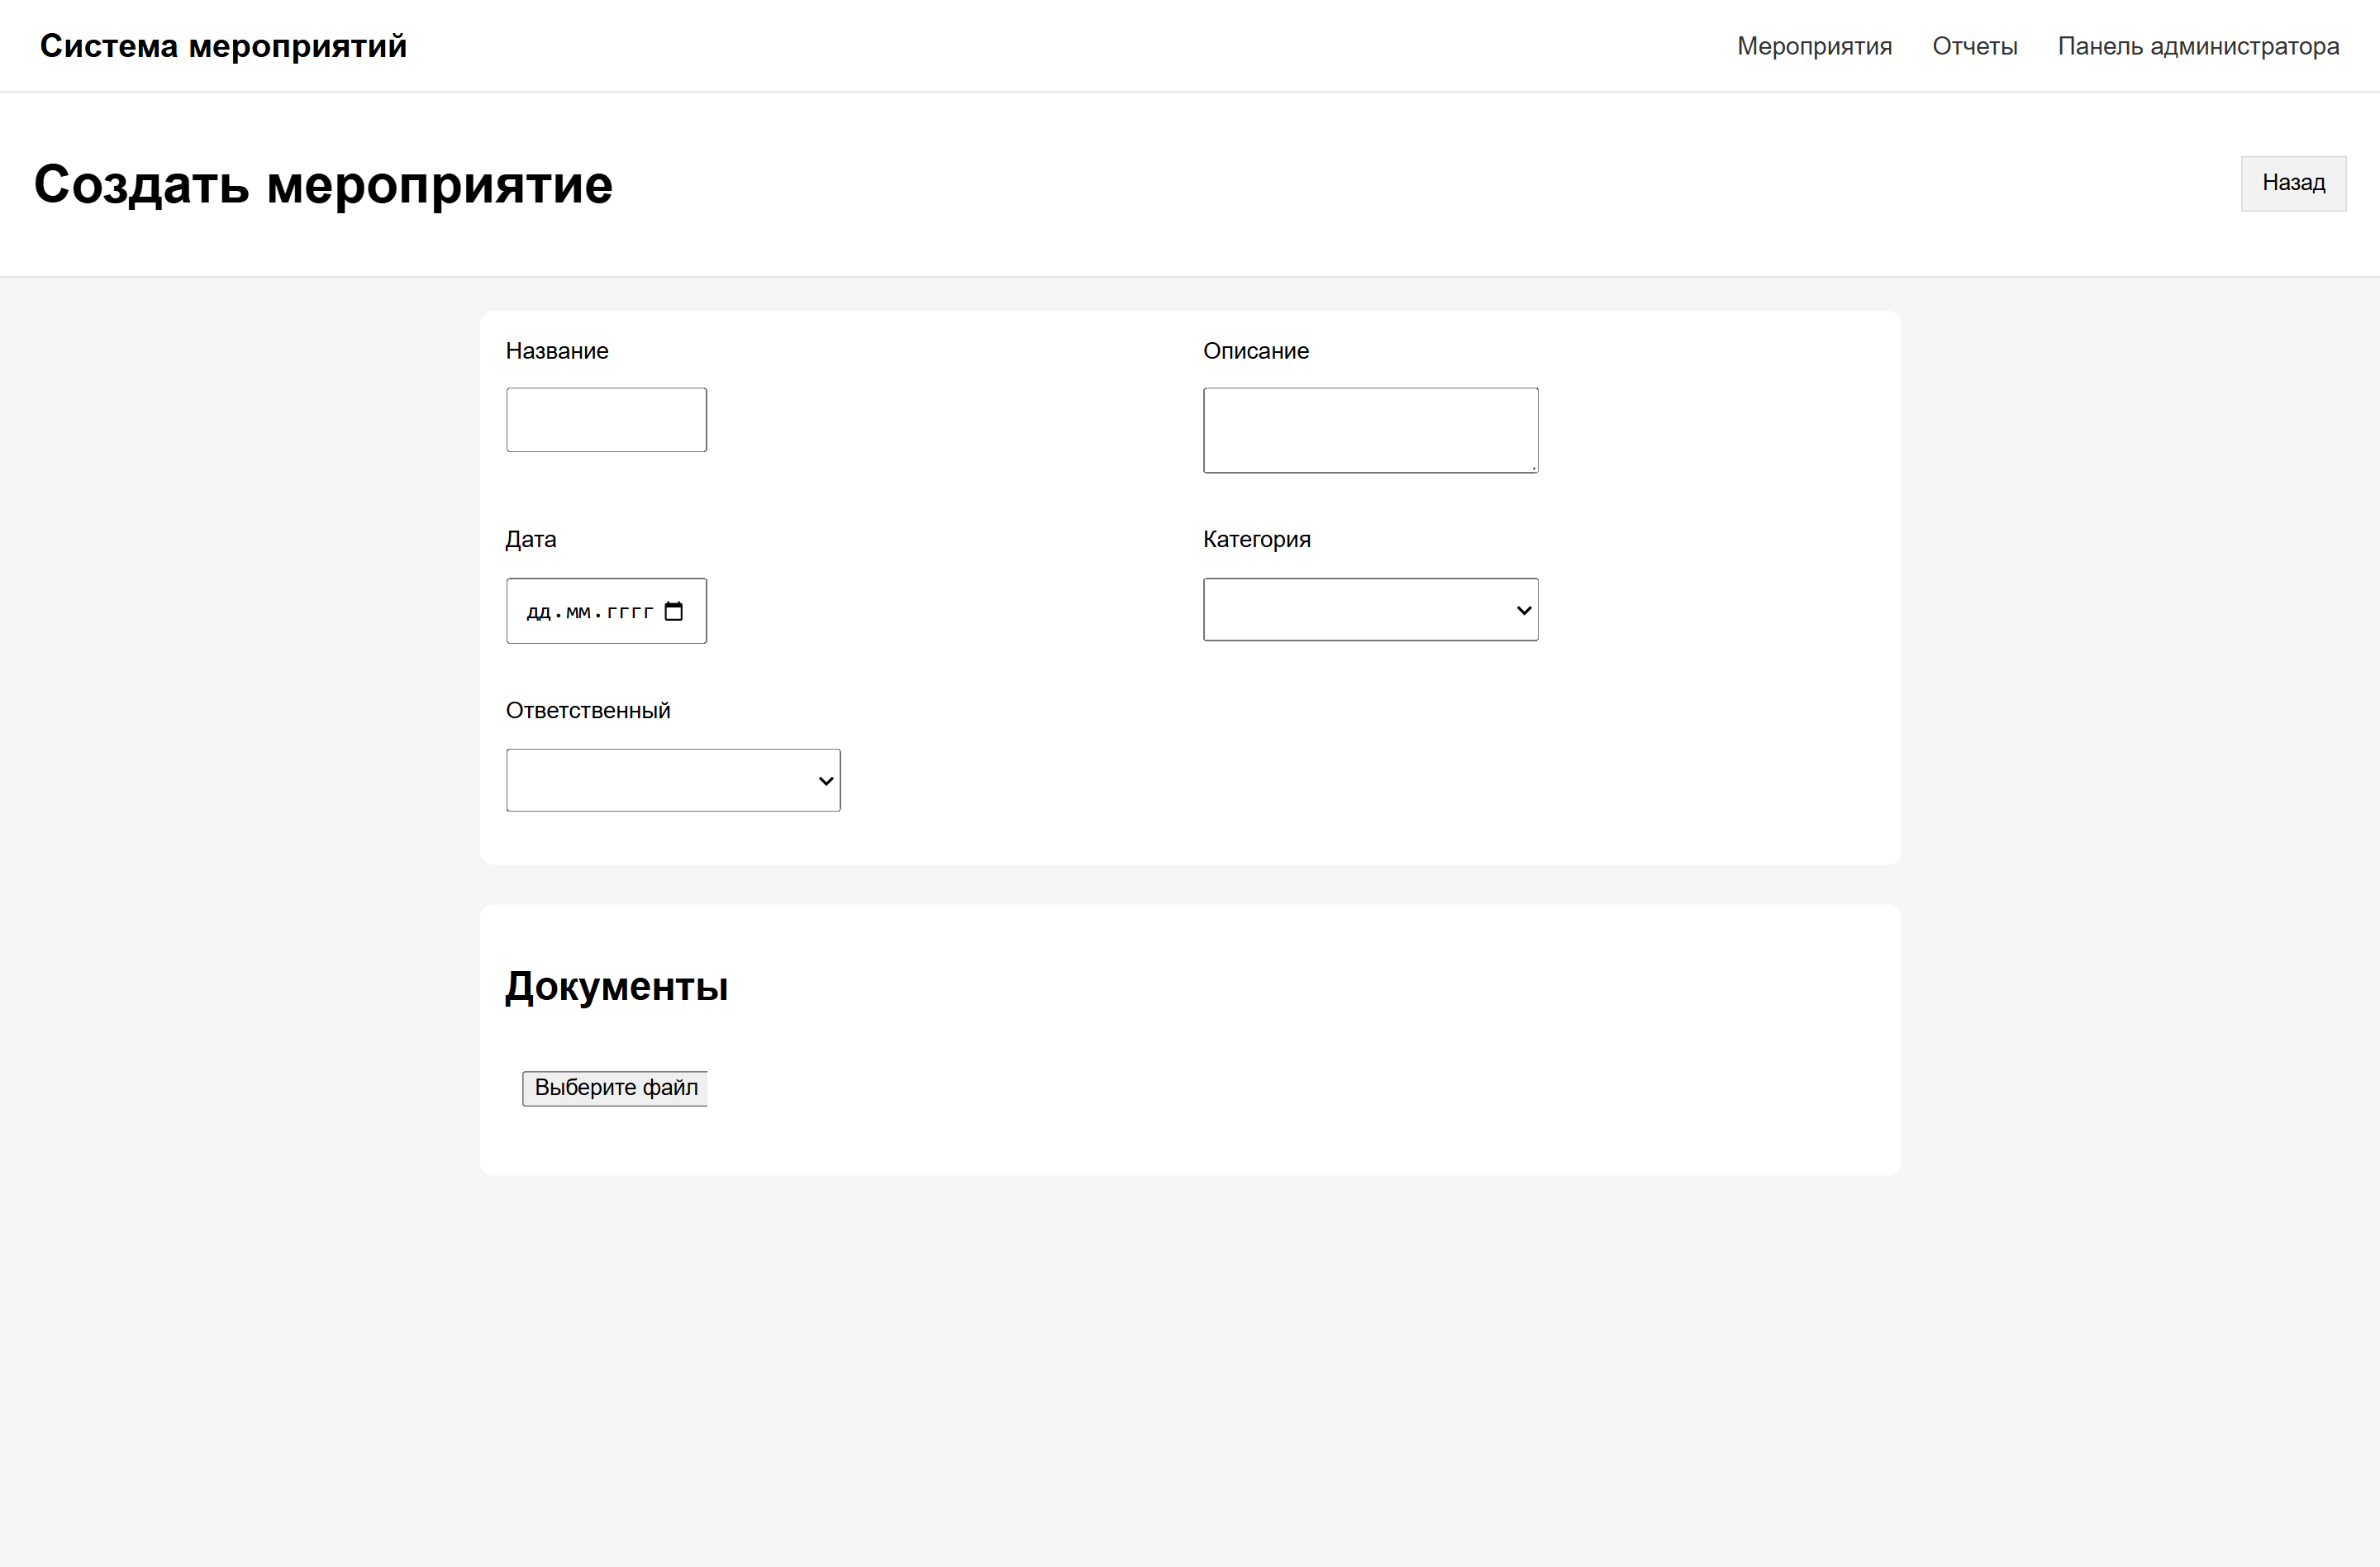
\includegraphics[width=0.95\textwidth]{images/create-event.png}
	\caption{Страница создания мероприятия}
	\label{fig:use_case}
\end{figure}
\begin{figure}[ht!]
	\centering
	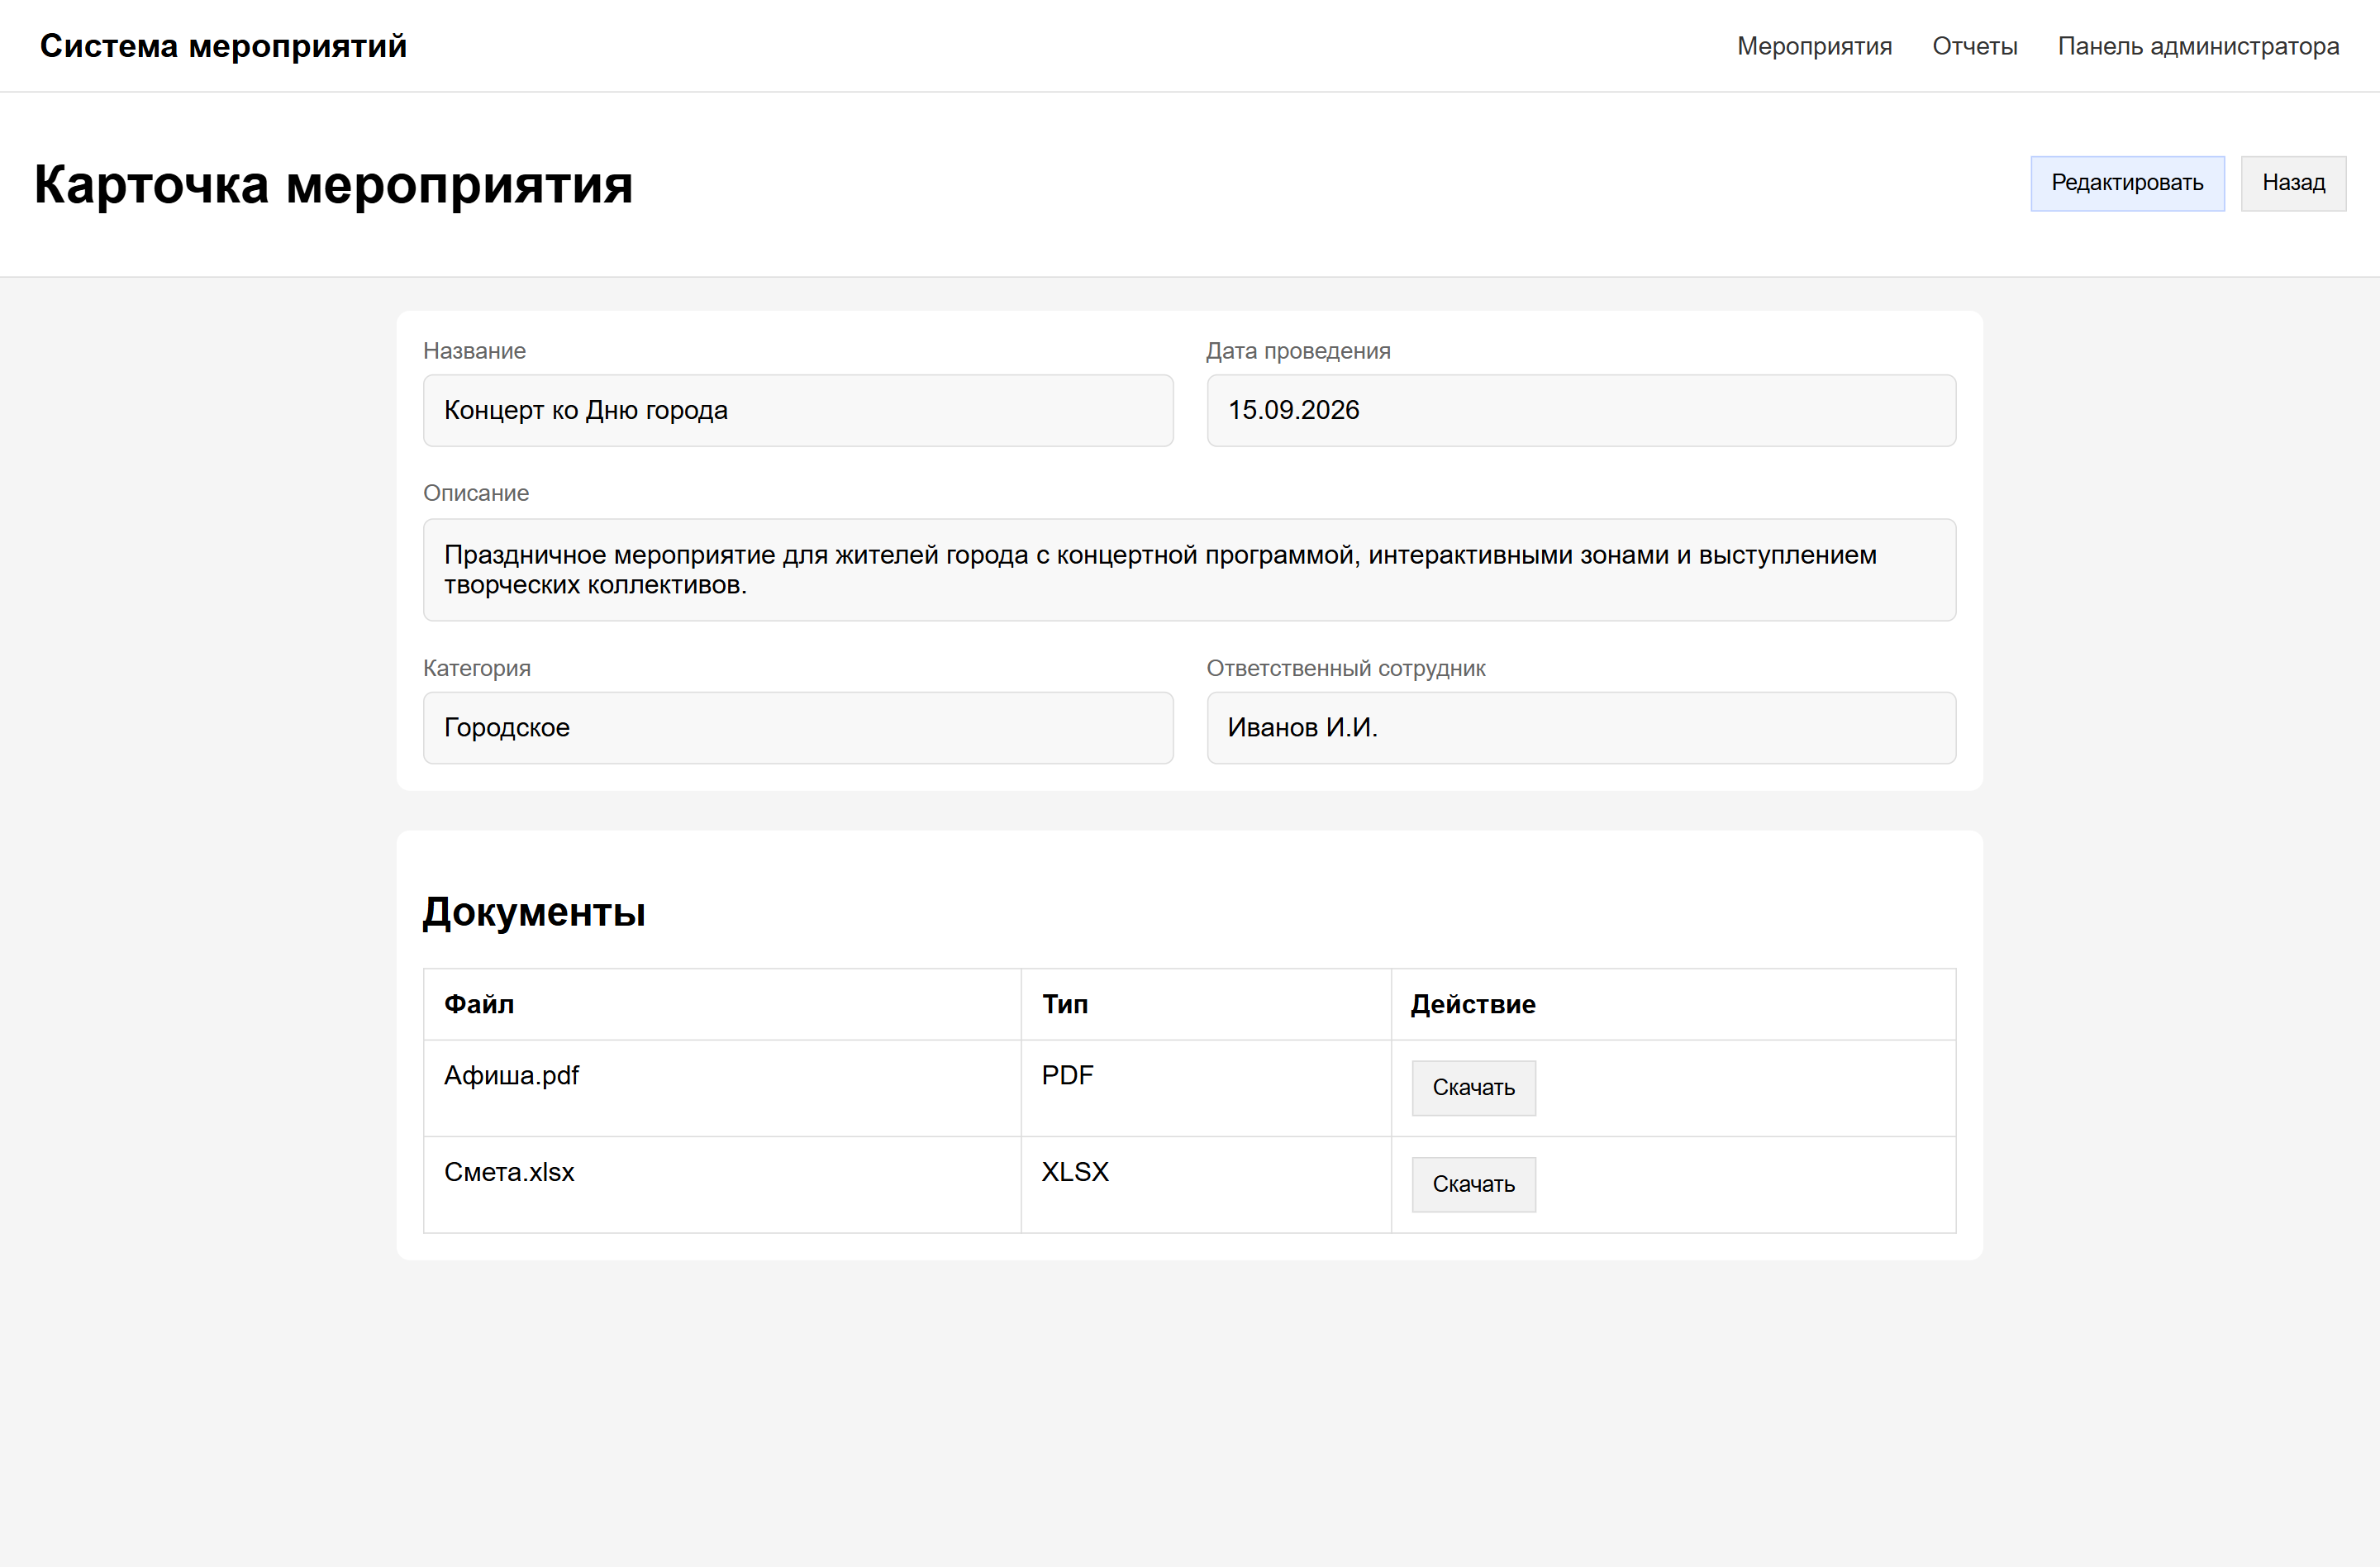
\includegraphics[width=0.95\textwidth]{images/event-view.png}
	\caption{Страница просмотра и редактирования мероприятия}
	\label{fig:use_case}
\end{figure}
\begin{figure}[ht!]
	\centering
	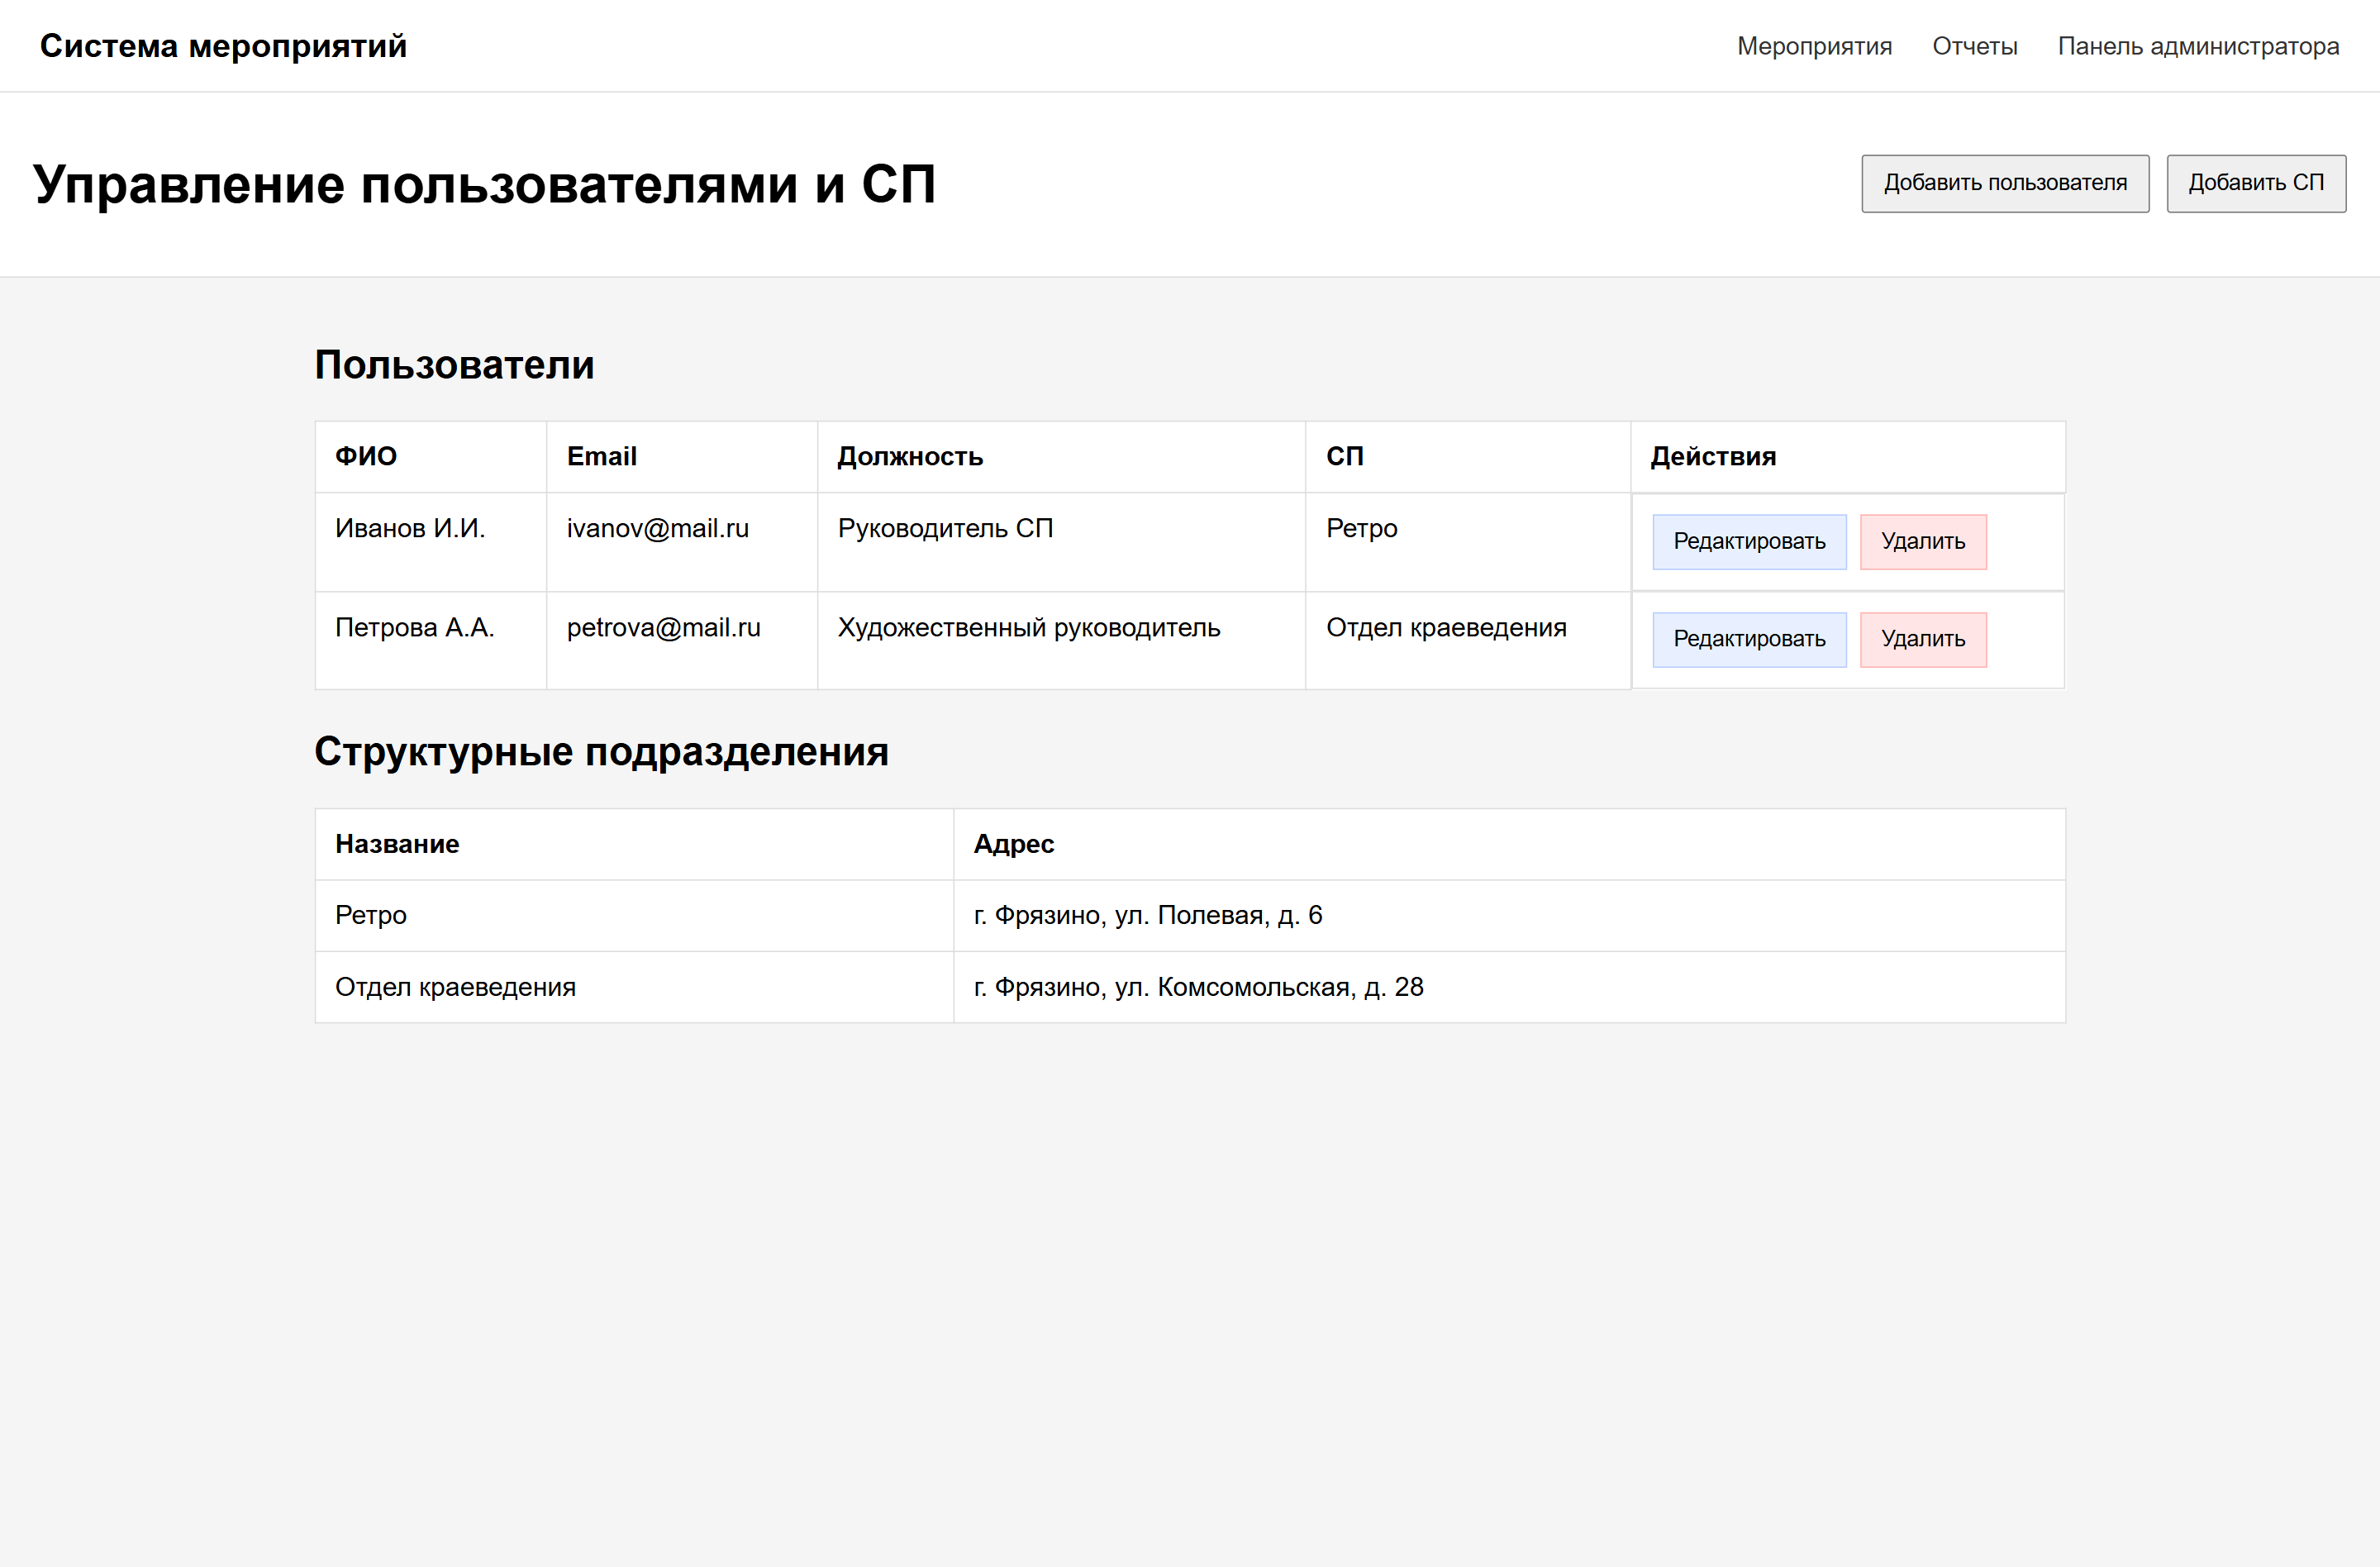
\includegraphics[width=0.95\textwidth]{images/users.png}
	\caption{Панель администратора}
	\label{fig:use_case}
\end{figure}
\begin{figure}[ht!]
	\centering
	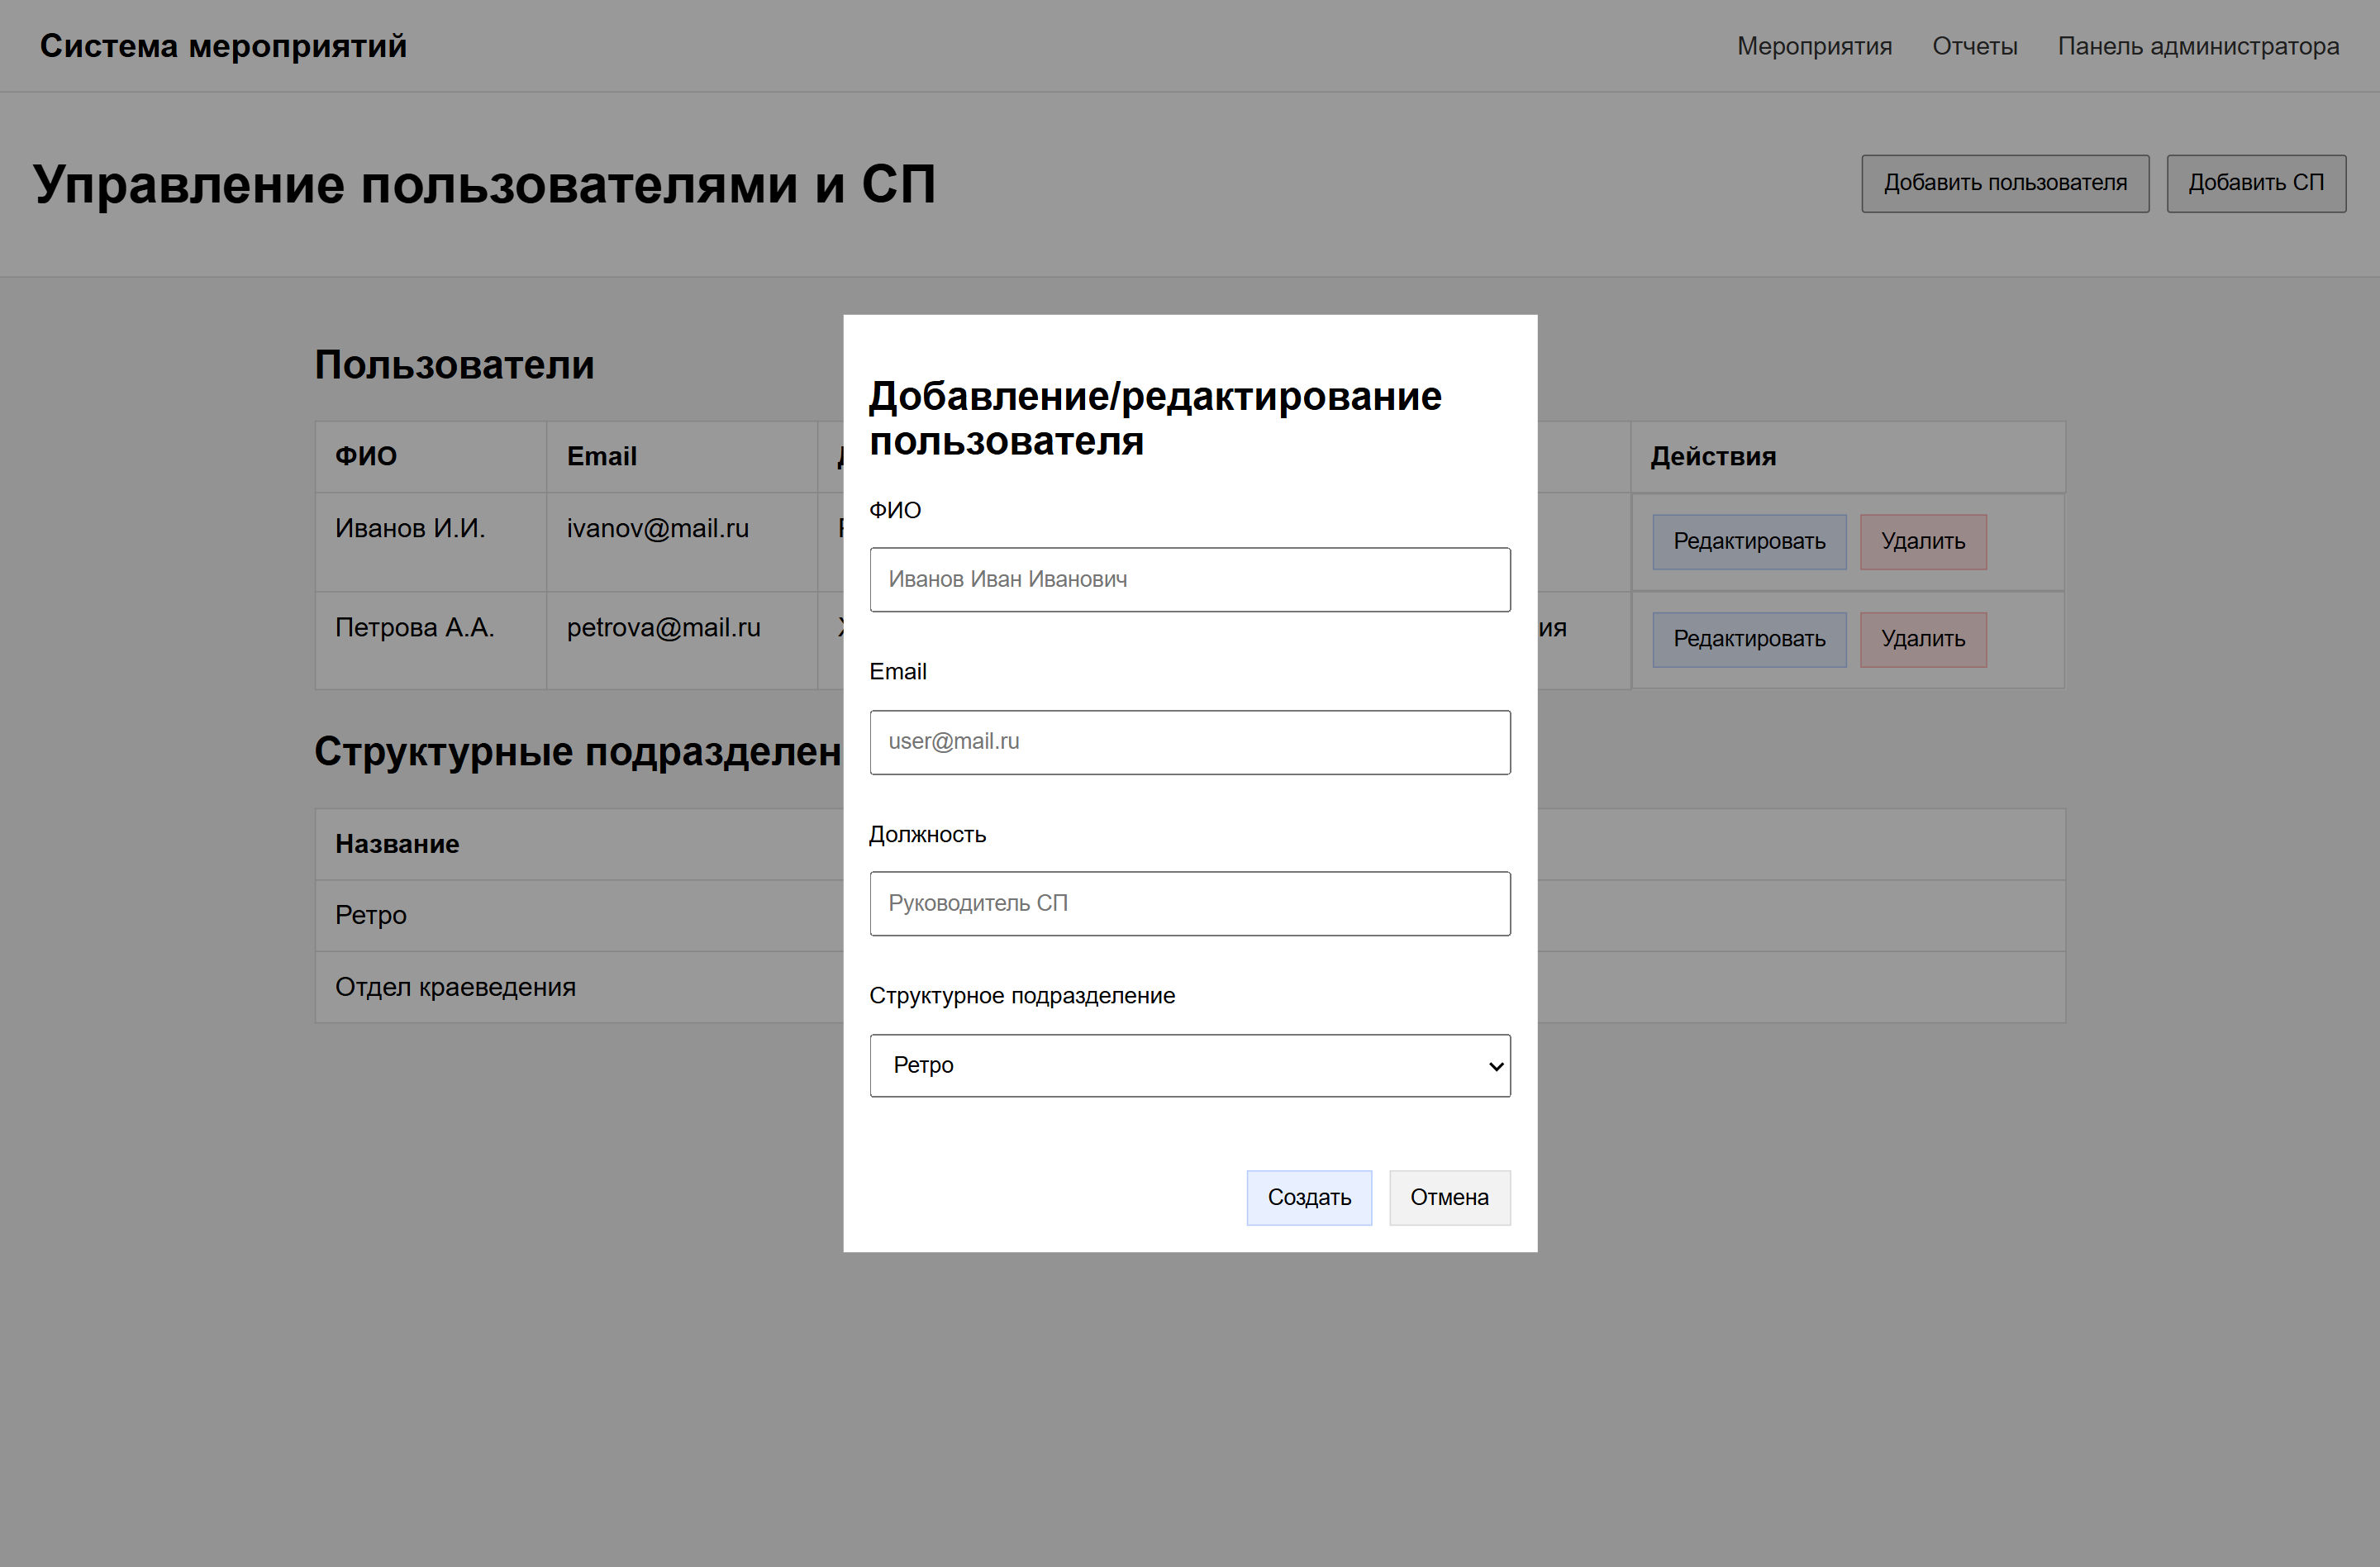
\includegraphics[width=0.95\textwidth]{images/create-edit-user.png}
	\caption{Панель администратора: добавление или редактирование пользователя}
	\label{fig:use_case}
\end{figure}
\begin{figure}[ht!]
	\centering
	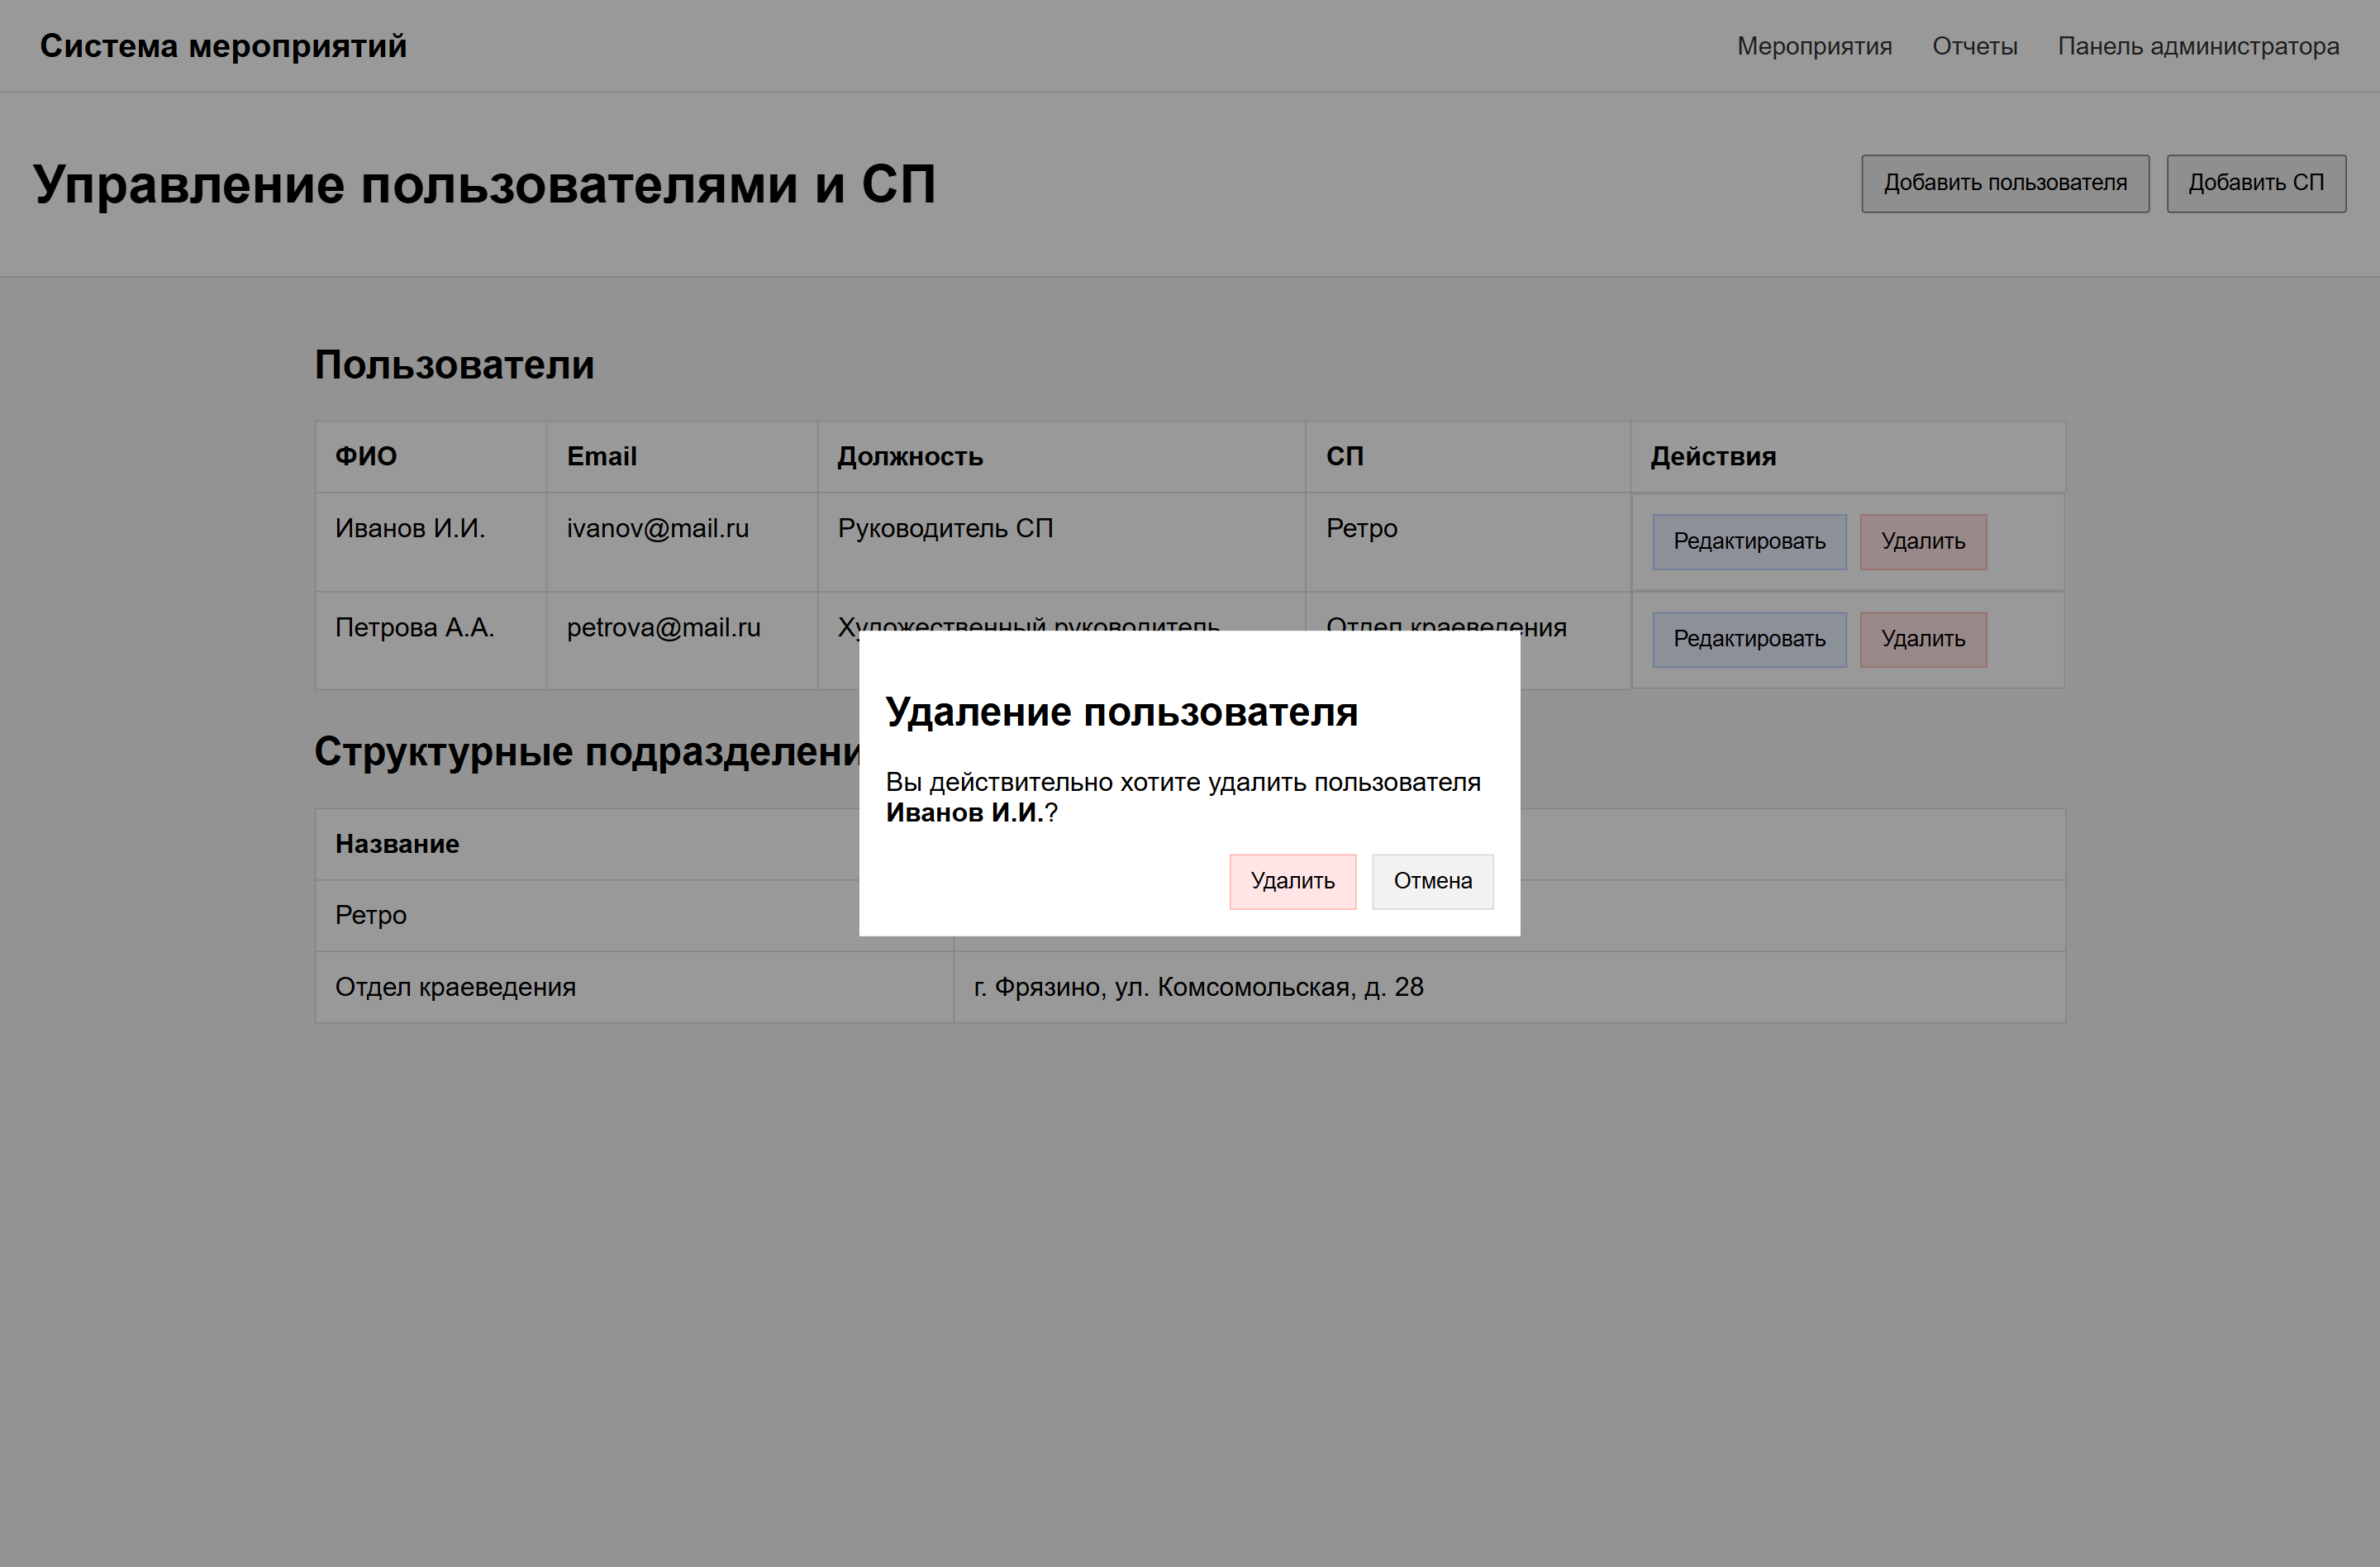
\includegraphics[width=0.95\textwidth]{images/delete-user.png}
	\caption{Панель администратора: удаление пользователя}
	\label{fig:use_case}
\end{figure}
\begin{figure}[ht!]
	\centering
	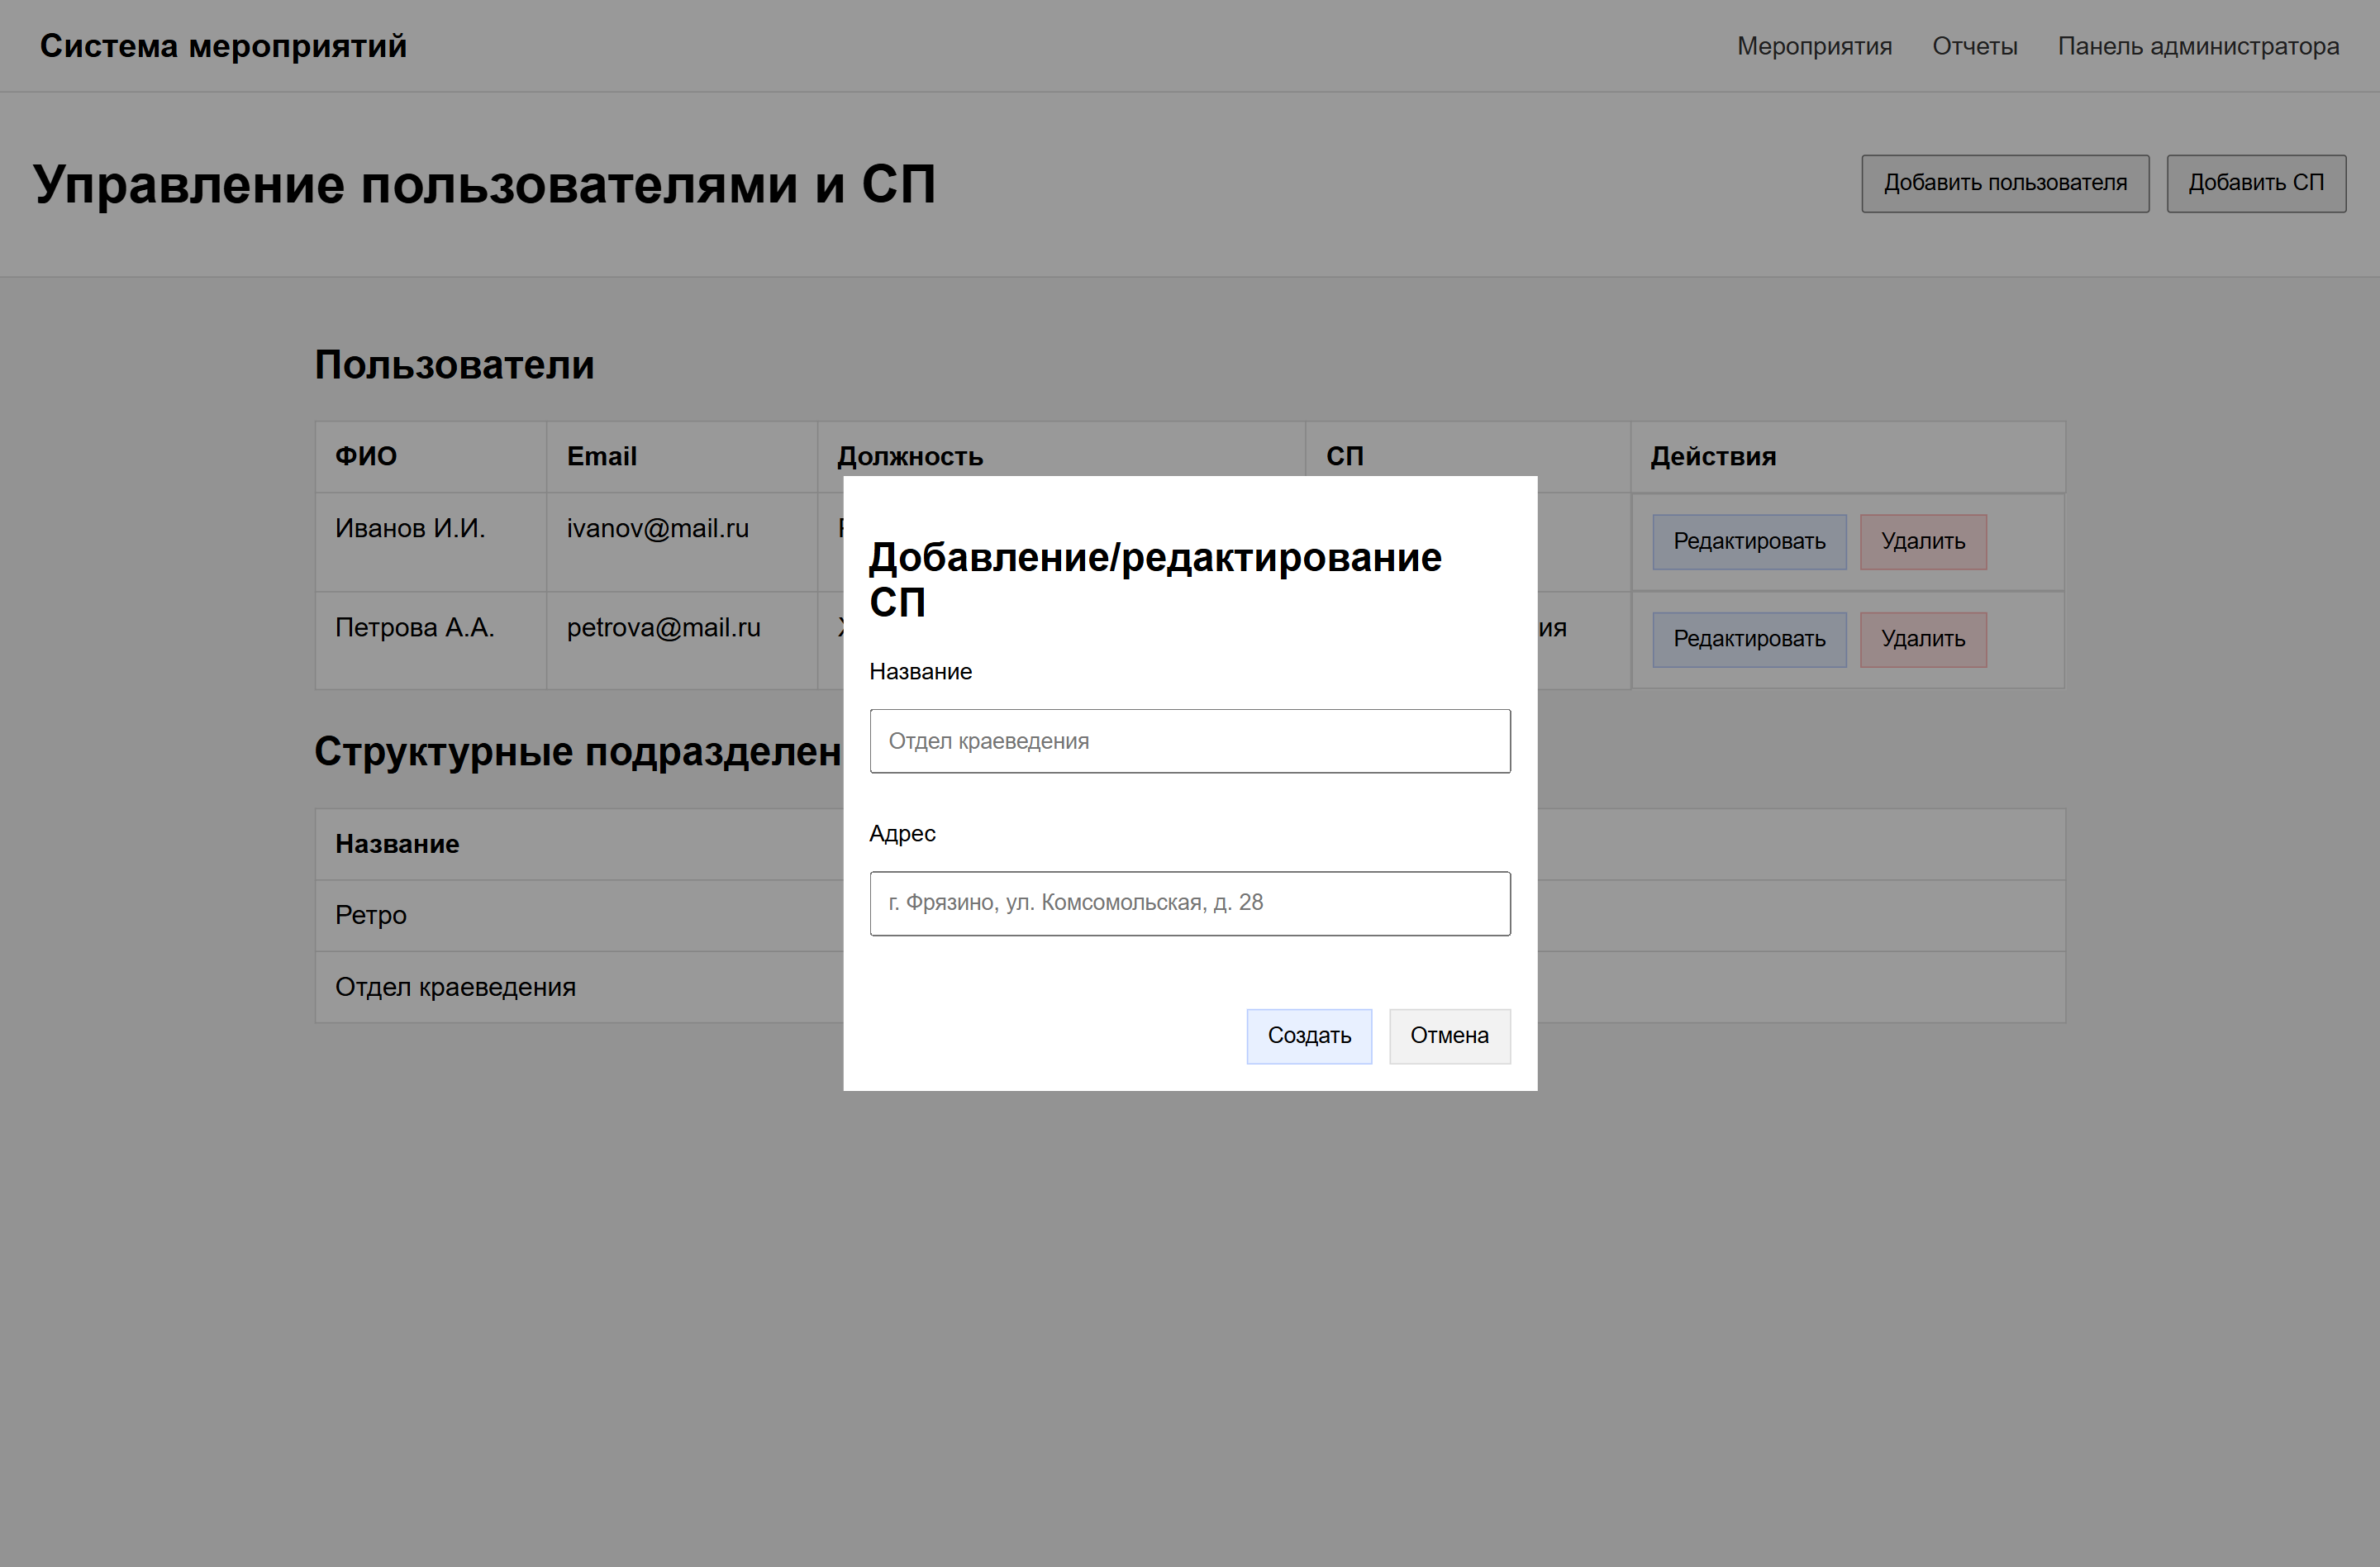
\includegraphics[width=0.95\textwidth]{images/create-edit-sp.png}
	\caption{Панель администратора: добавление или редактирование структурного подразделения}
	\label{fig:use_case}
\end{figure}
\begin{figure}[ht!]
	\centering
	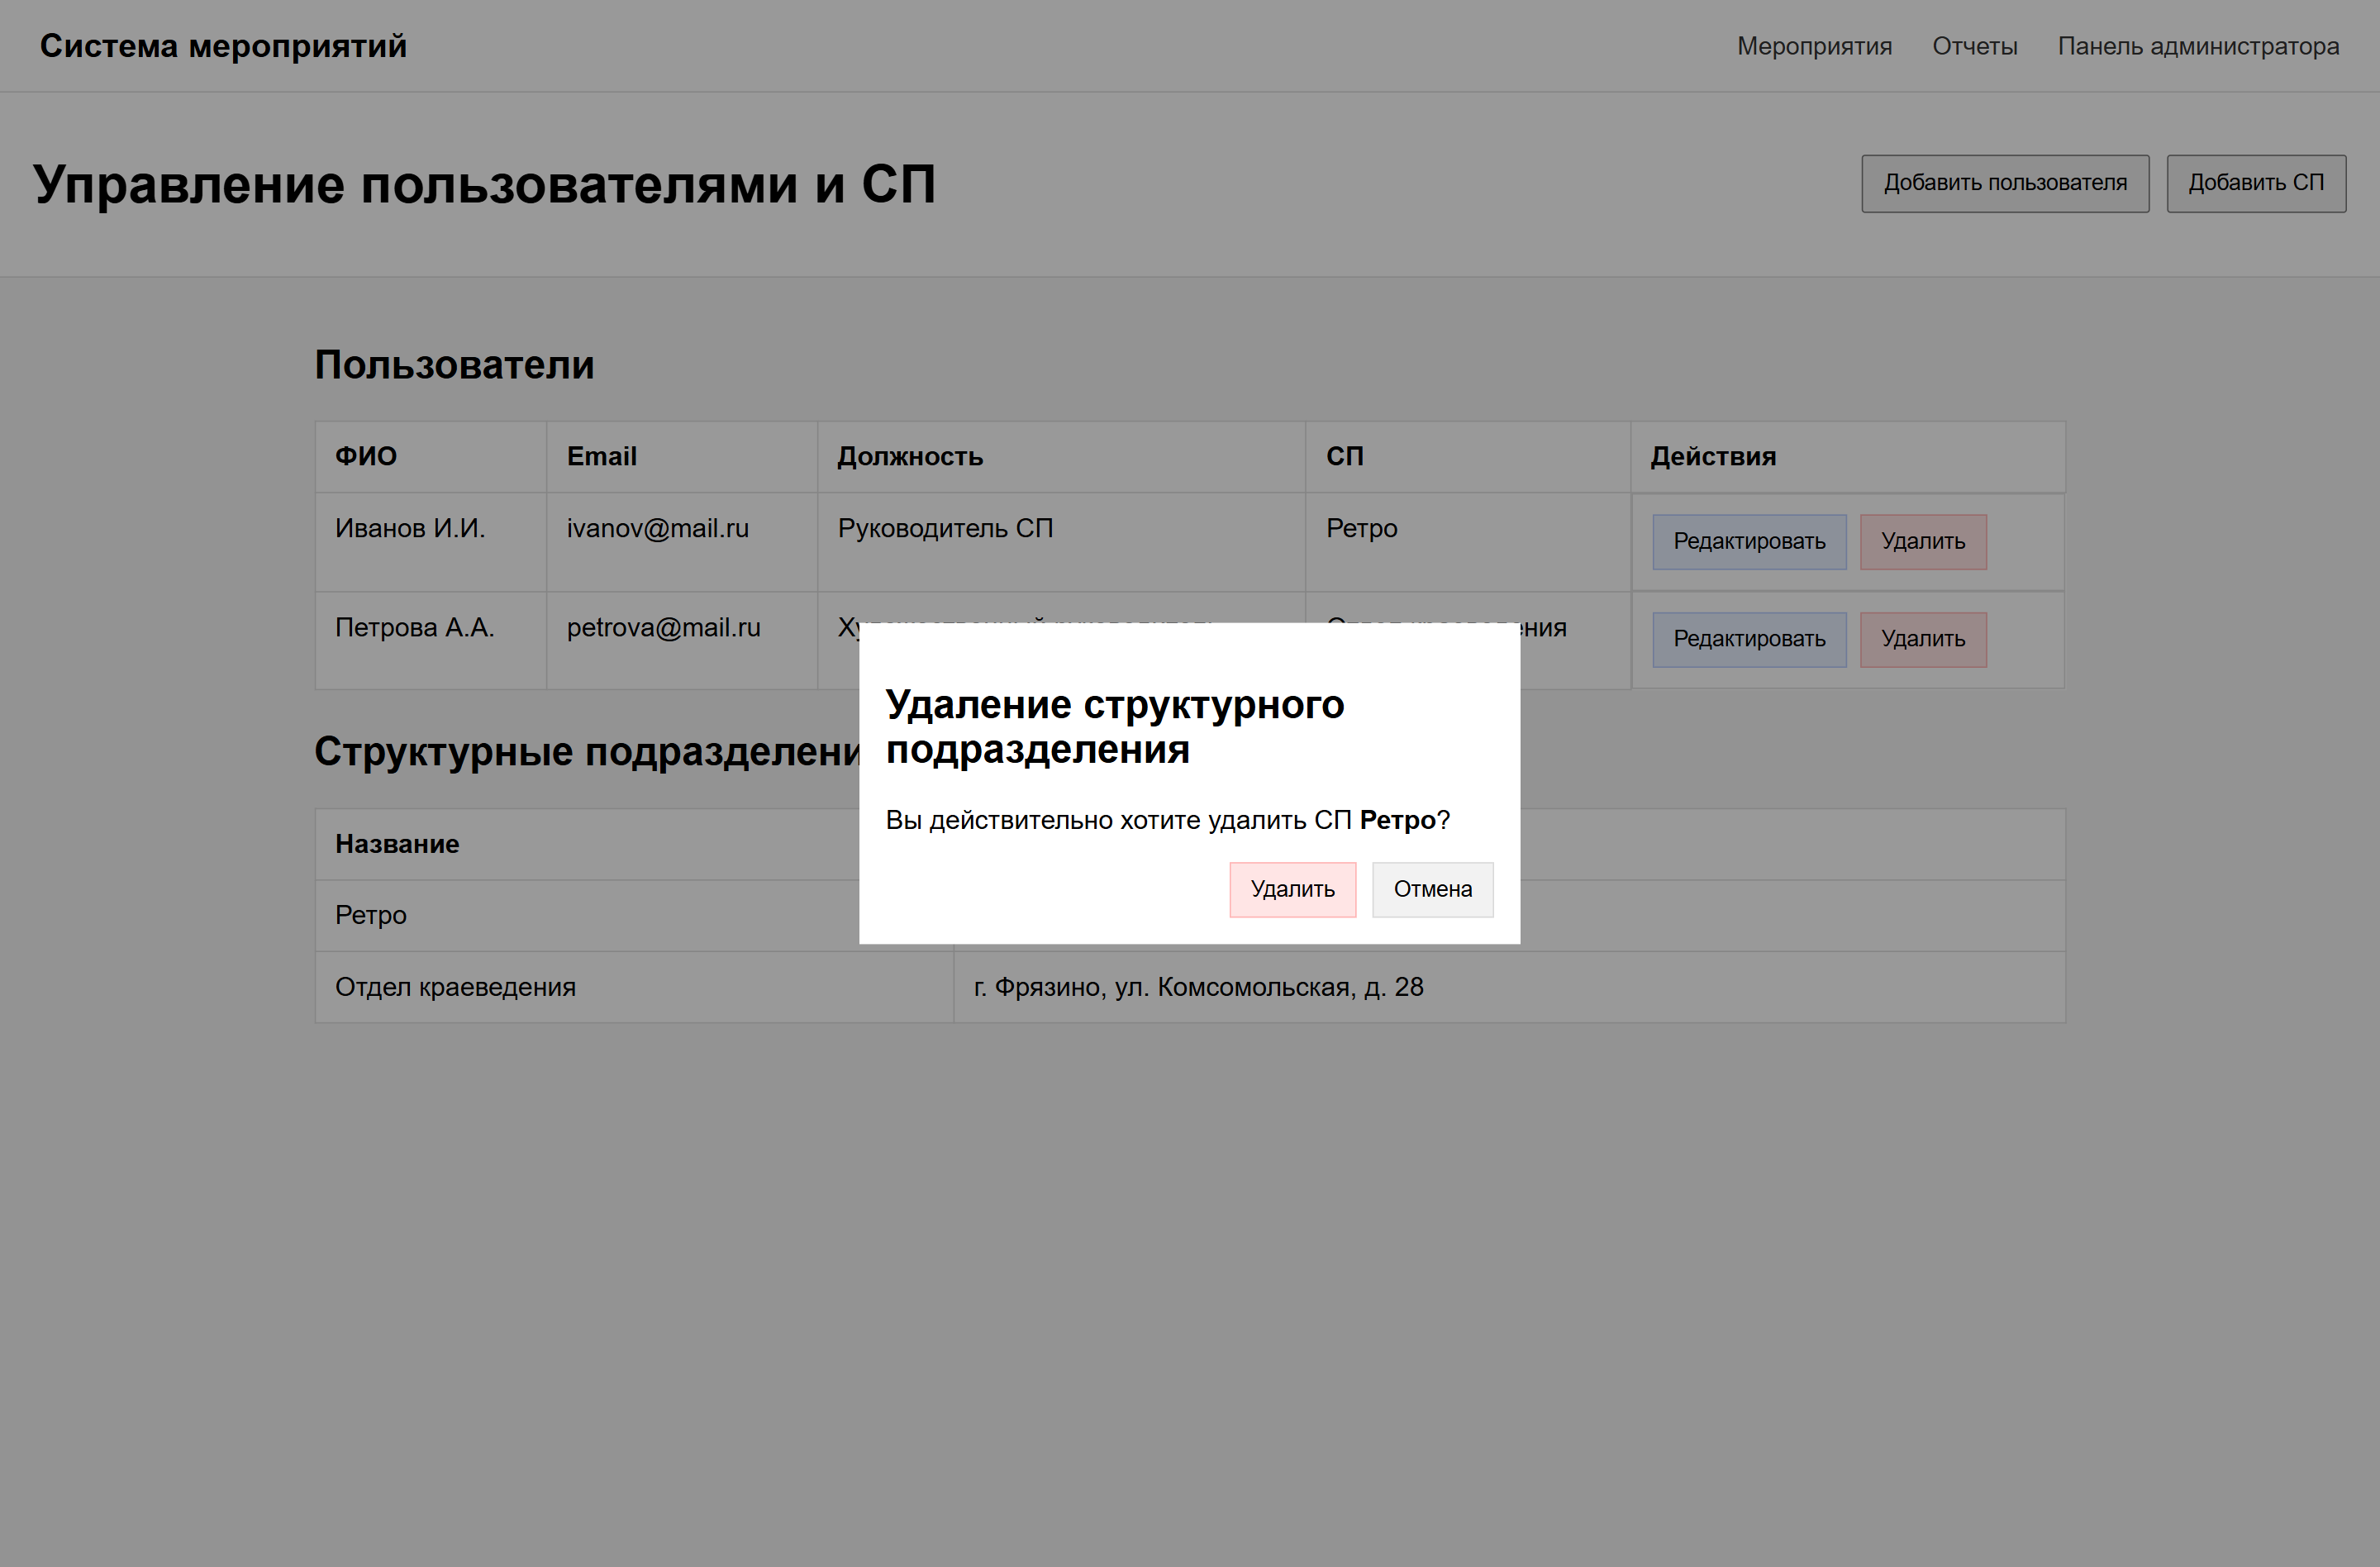
\includegraphics[width=0.95\textwidth]{images/delete-sp.png}
	\caption{Панель администратора: удаление структурного подразделения}
	\label{fig:use_case}
\end{figure}
\begin{figure}[ht!]
	\centering
	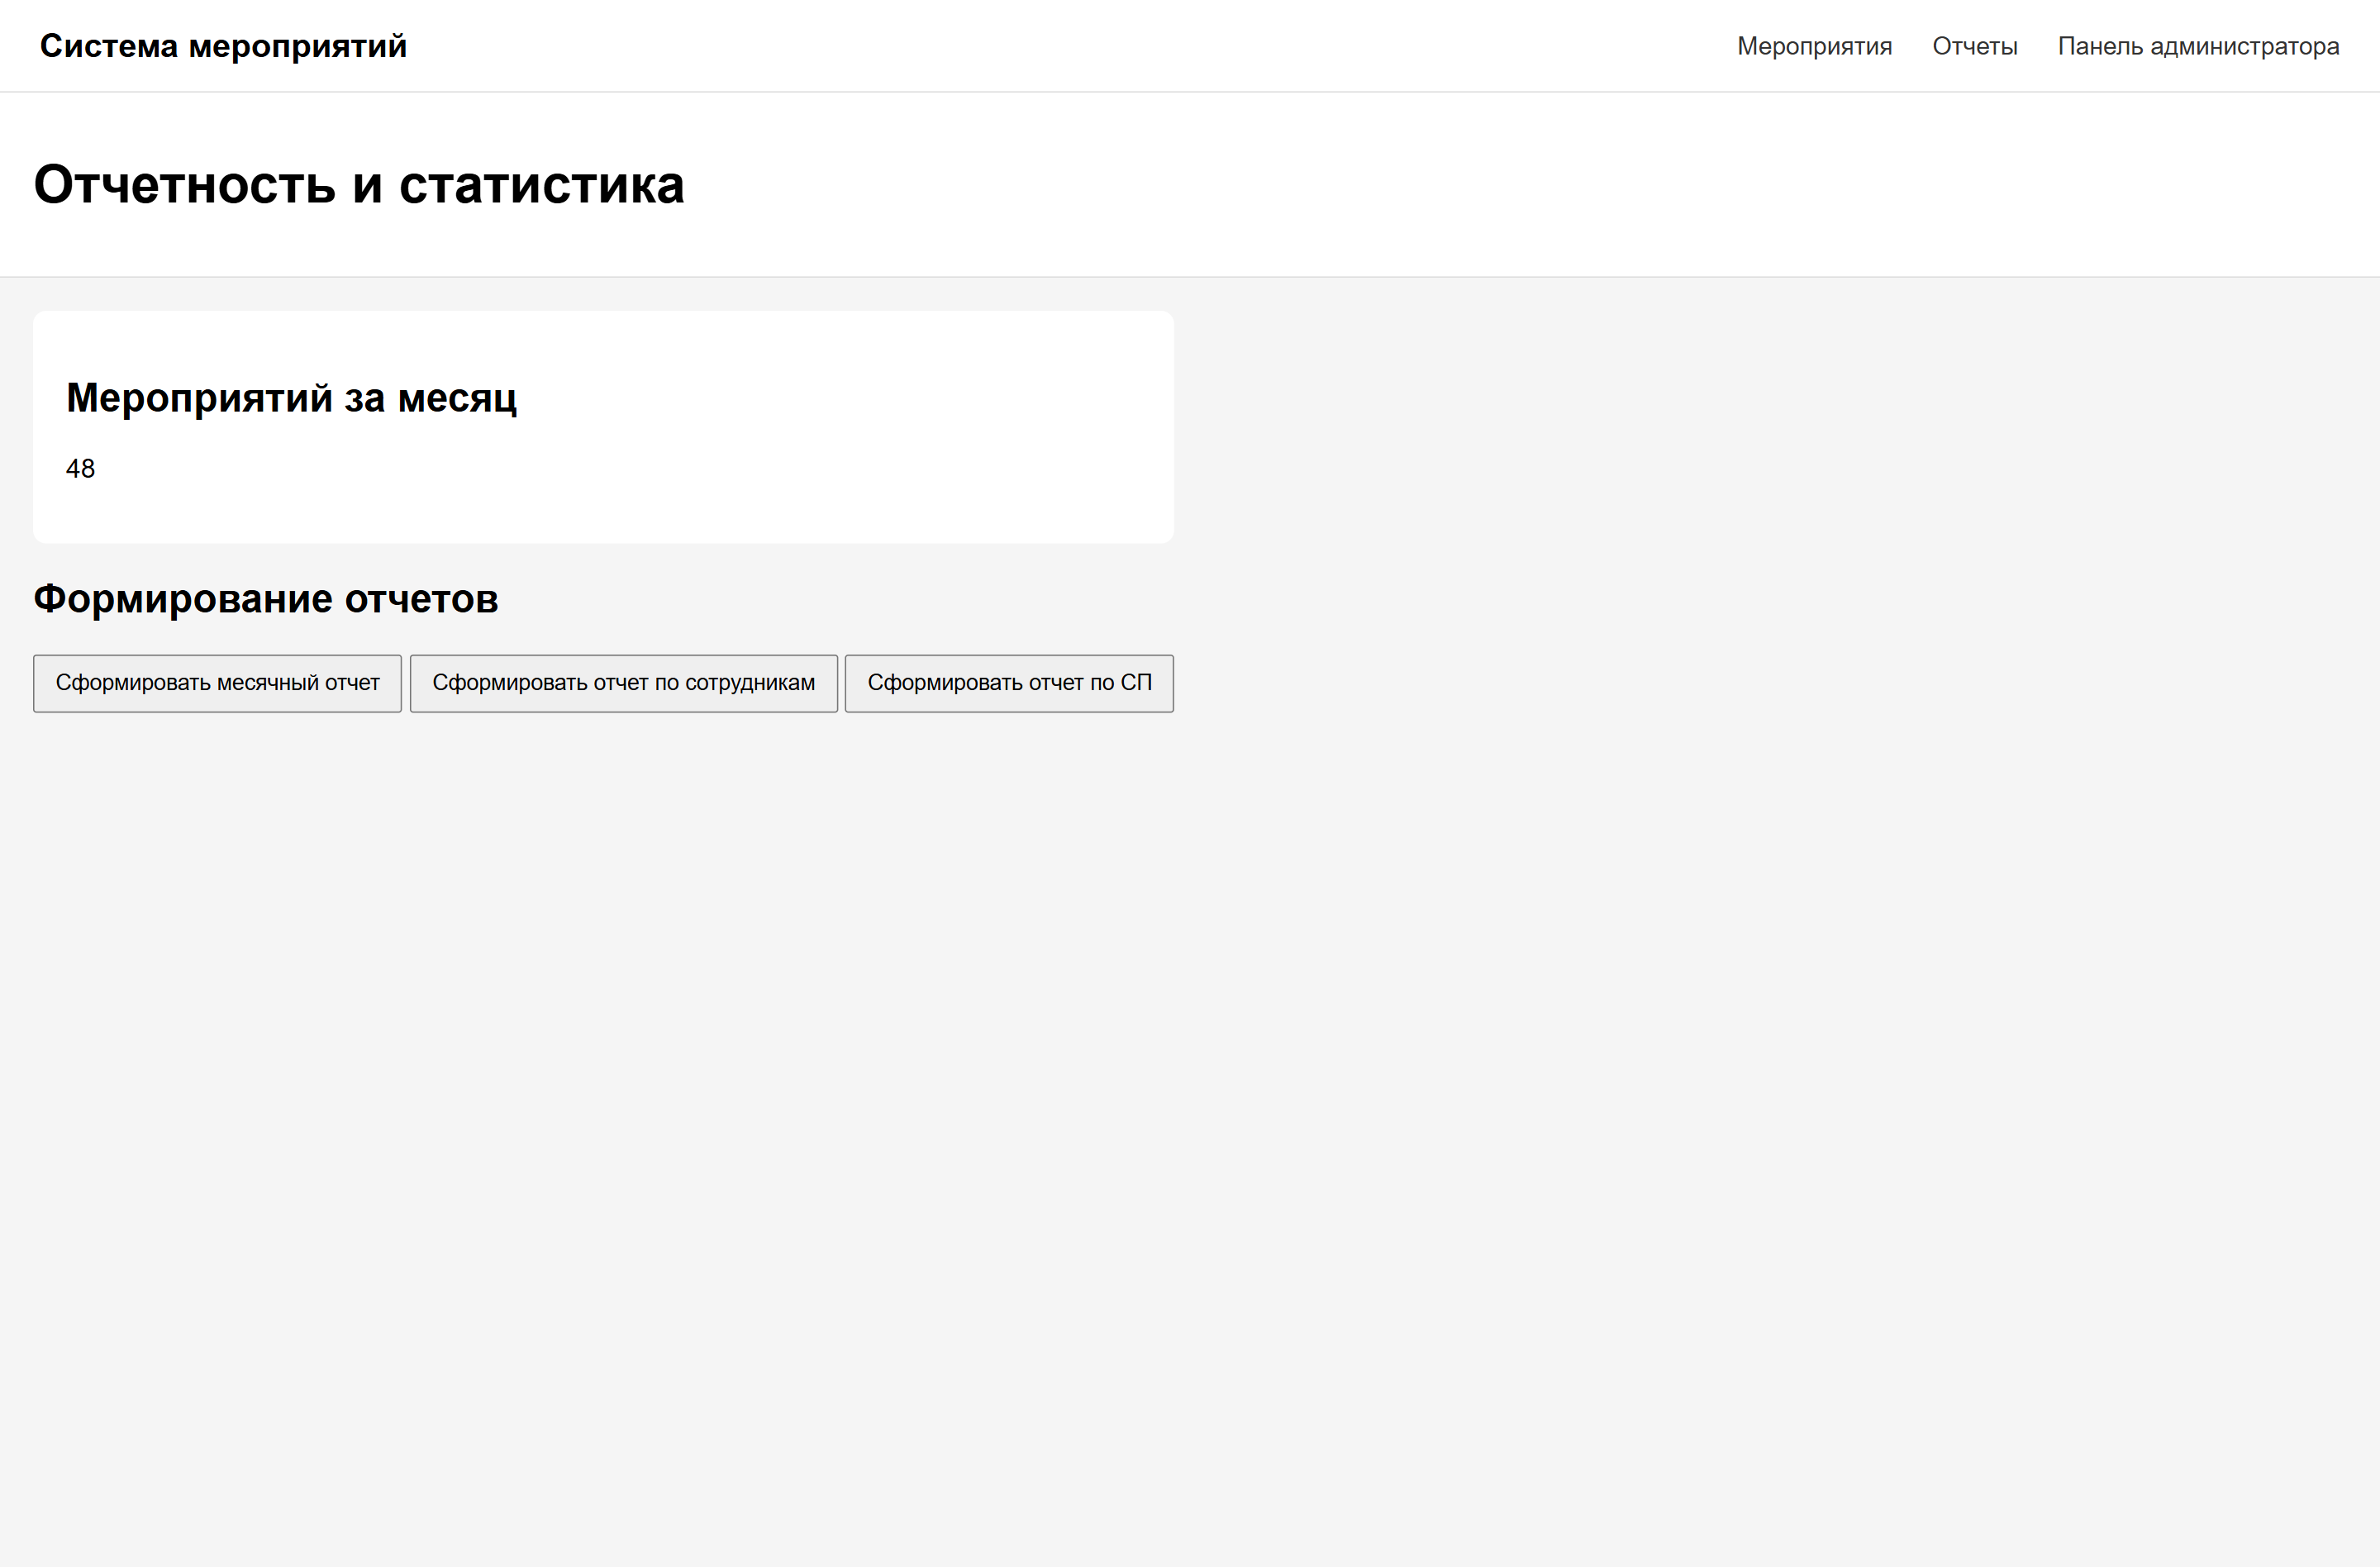
\includegraphics[width=0.95\textwidth]{images/reports.png}
	\caption{Страница выгрузки отчетов}
	\label{fig:use_case}
\end{figure}
